\chapter{背景估计}\label{chap:bkg_estimation}
4W物理分析背景分为可以贡献两个相同电荷的过程(promptSS),电荷误鉴别(QmisID)和“假”轻子过程(fakes)。
promptSS主要来自$t\bar{t}V$, $VV$, $tV$以及$t\bar{t}H$过程,该背景可用MC估计。
QmisID一般来自于$Z+jets$和$t\bar{t}$(轻子衰变过程)。
fakes来自于$W+jets$,$t\bar{t}$(半轻子衰变)过程,其中一个jet被误判成轻子或者一个轻子来源于\bjet (non-prompt)。
目前ATLAS MC不能很好地描述QmisID和fakes,如图~\ref{fig:nominal:datavspureMC}所示,如果所有背景均用MC模拟,可以看到,数据跟预期有非常大的偏差。
所以,这表明data-driven的方法去估计QmisID和fakes是有必要的。在以下章节中,将分别讲述QmisID和fakes的估计方法。
\begin{figure}[h]
\begin{minipage}[t]{0.3\linewidth}
 \centering
 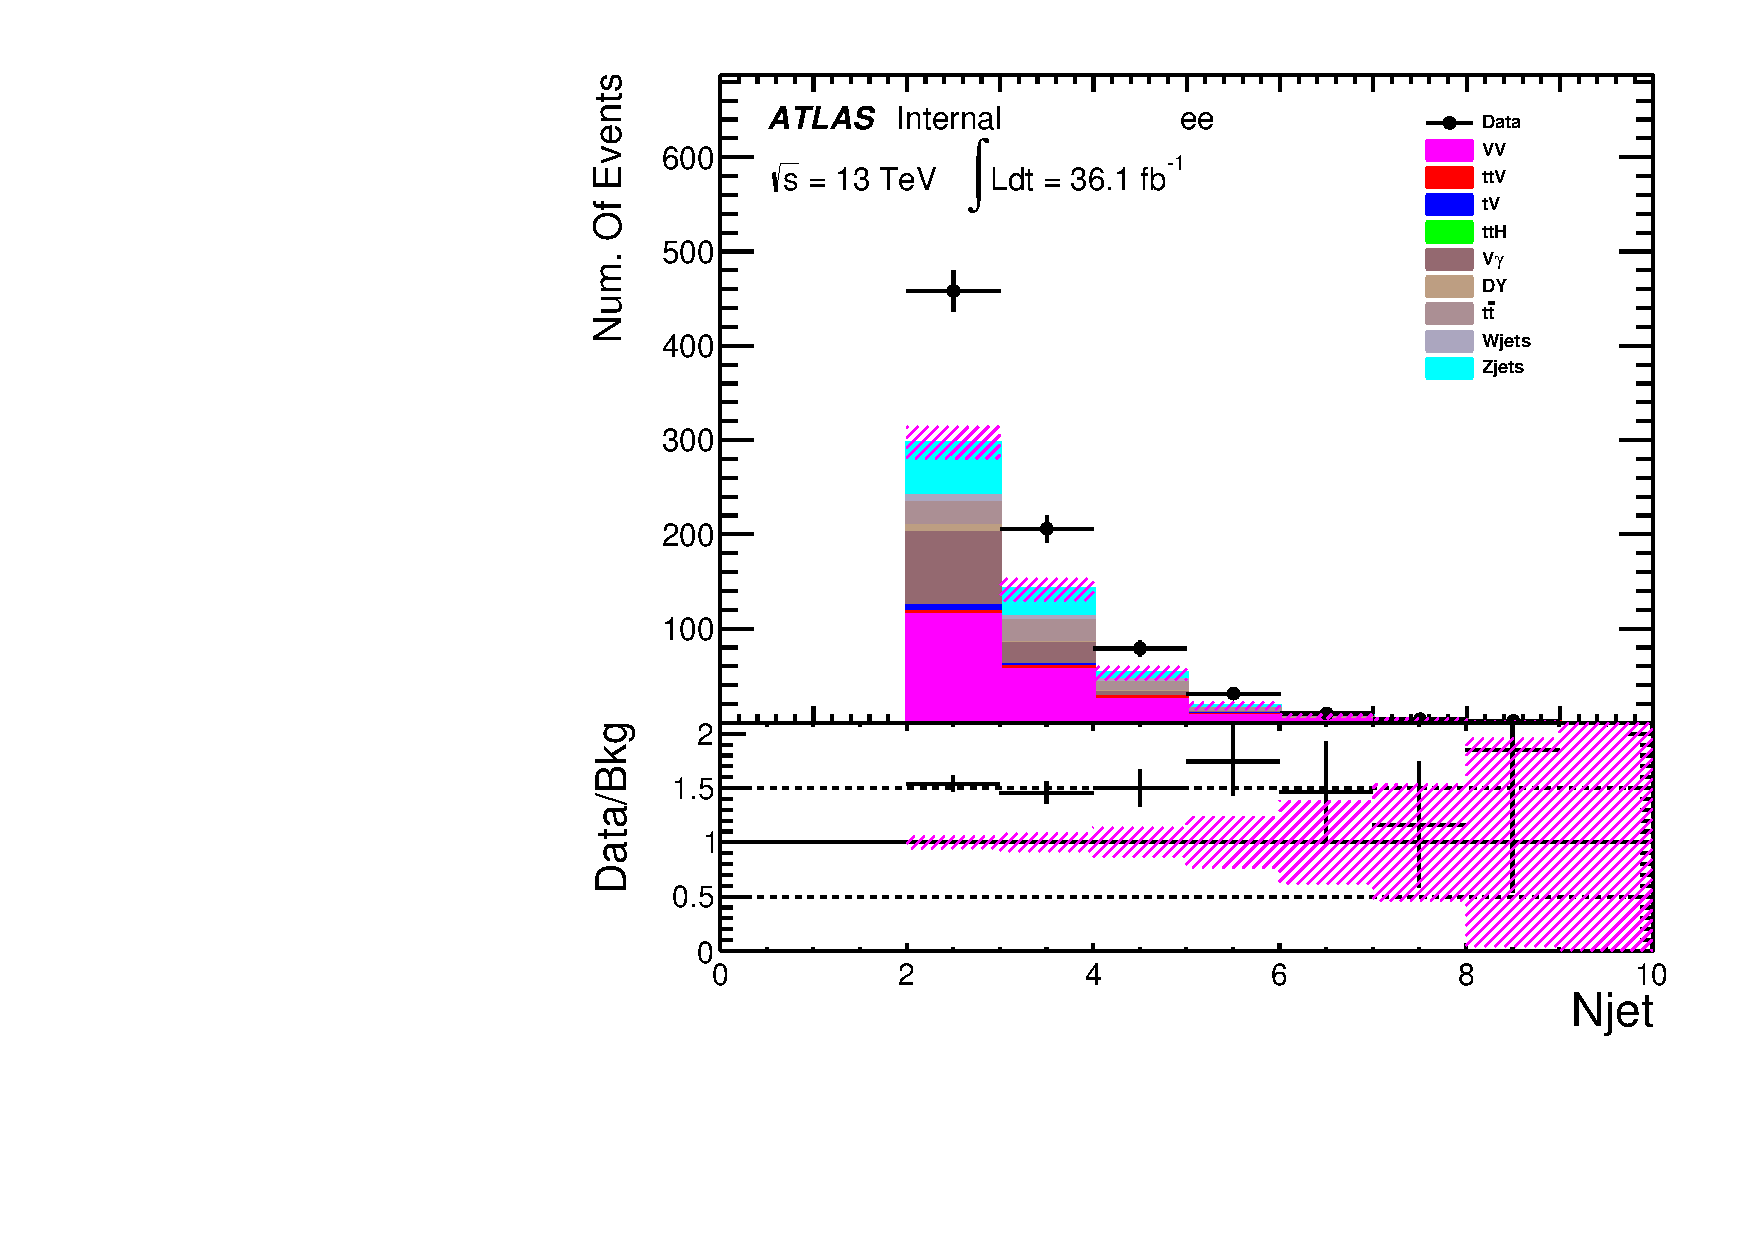
\includegraphics[width=1.0\textwidth,angle=-90]{fig/nominal/numOfjet_ee.pdf}
 \label{fig:nominal:numOfjet_ee.pdf}
 \end{minipage}
\begin{minipage}[t]{0.3\linewidth}
 \centering
 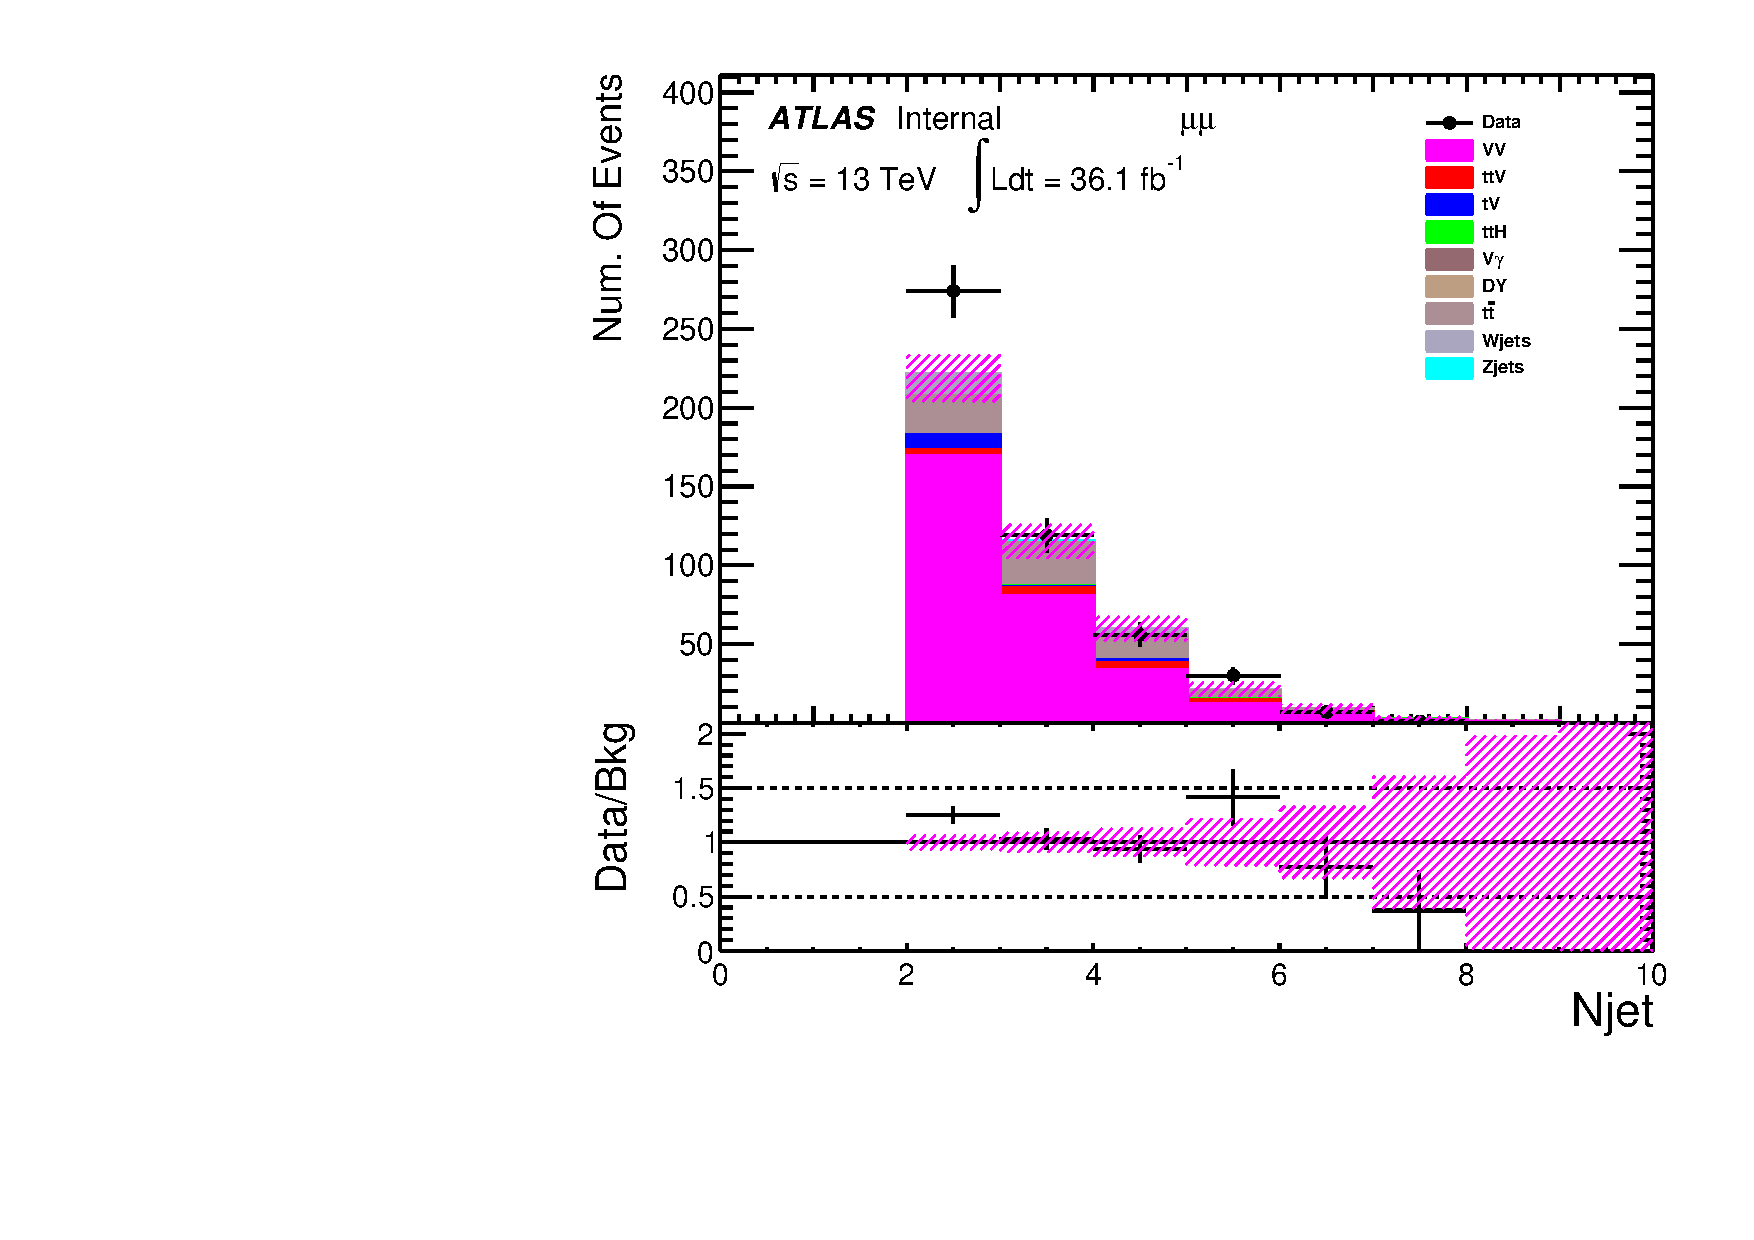
\includegraphics[width=1.0\textwidth,angle=-90]{fig/nominal/numOfjet_mumu.pdf}
 \label{fig:nominal:numOfjet_mumu.pdf}
 \end{minipage}
\begin{minipage}[t]{0.3\linewidth}
 \centering
 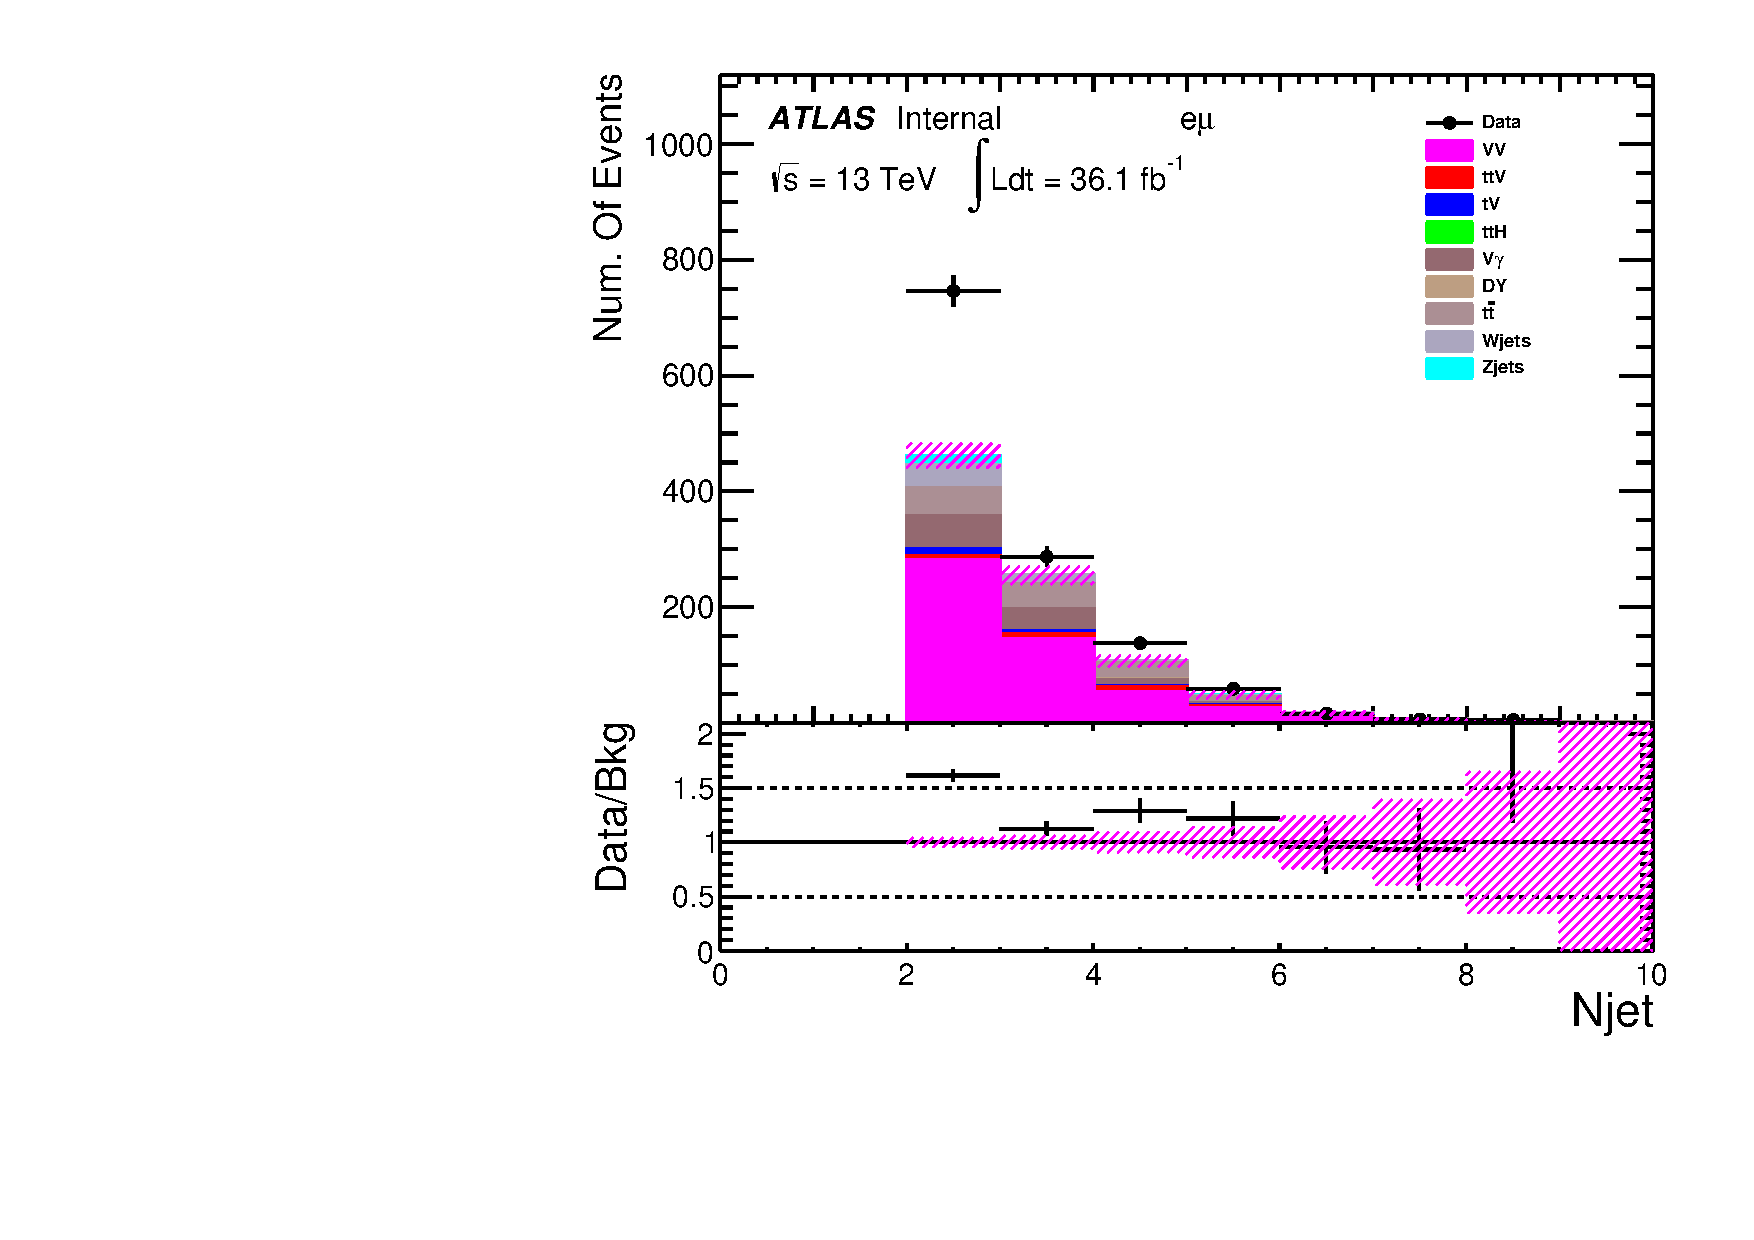
\includegraphics[width=1.0\textwidth,angle=-90]{fig/nominal/numOfjet_emu.pdf}
 \label{fig:nominal:numOfjet_emu.pdf}
 \end{minipage}
\begin{minipage}[t]{0.3\linewidth}
 \centering
 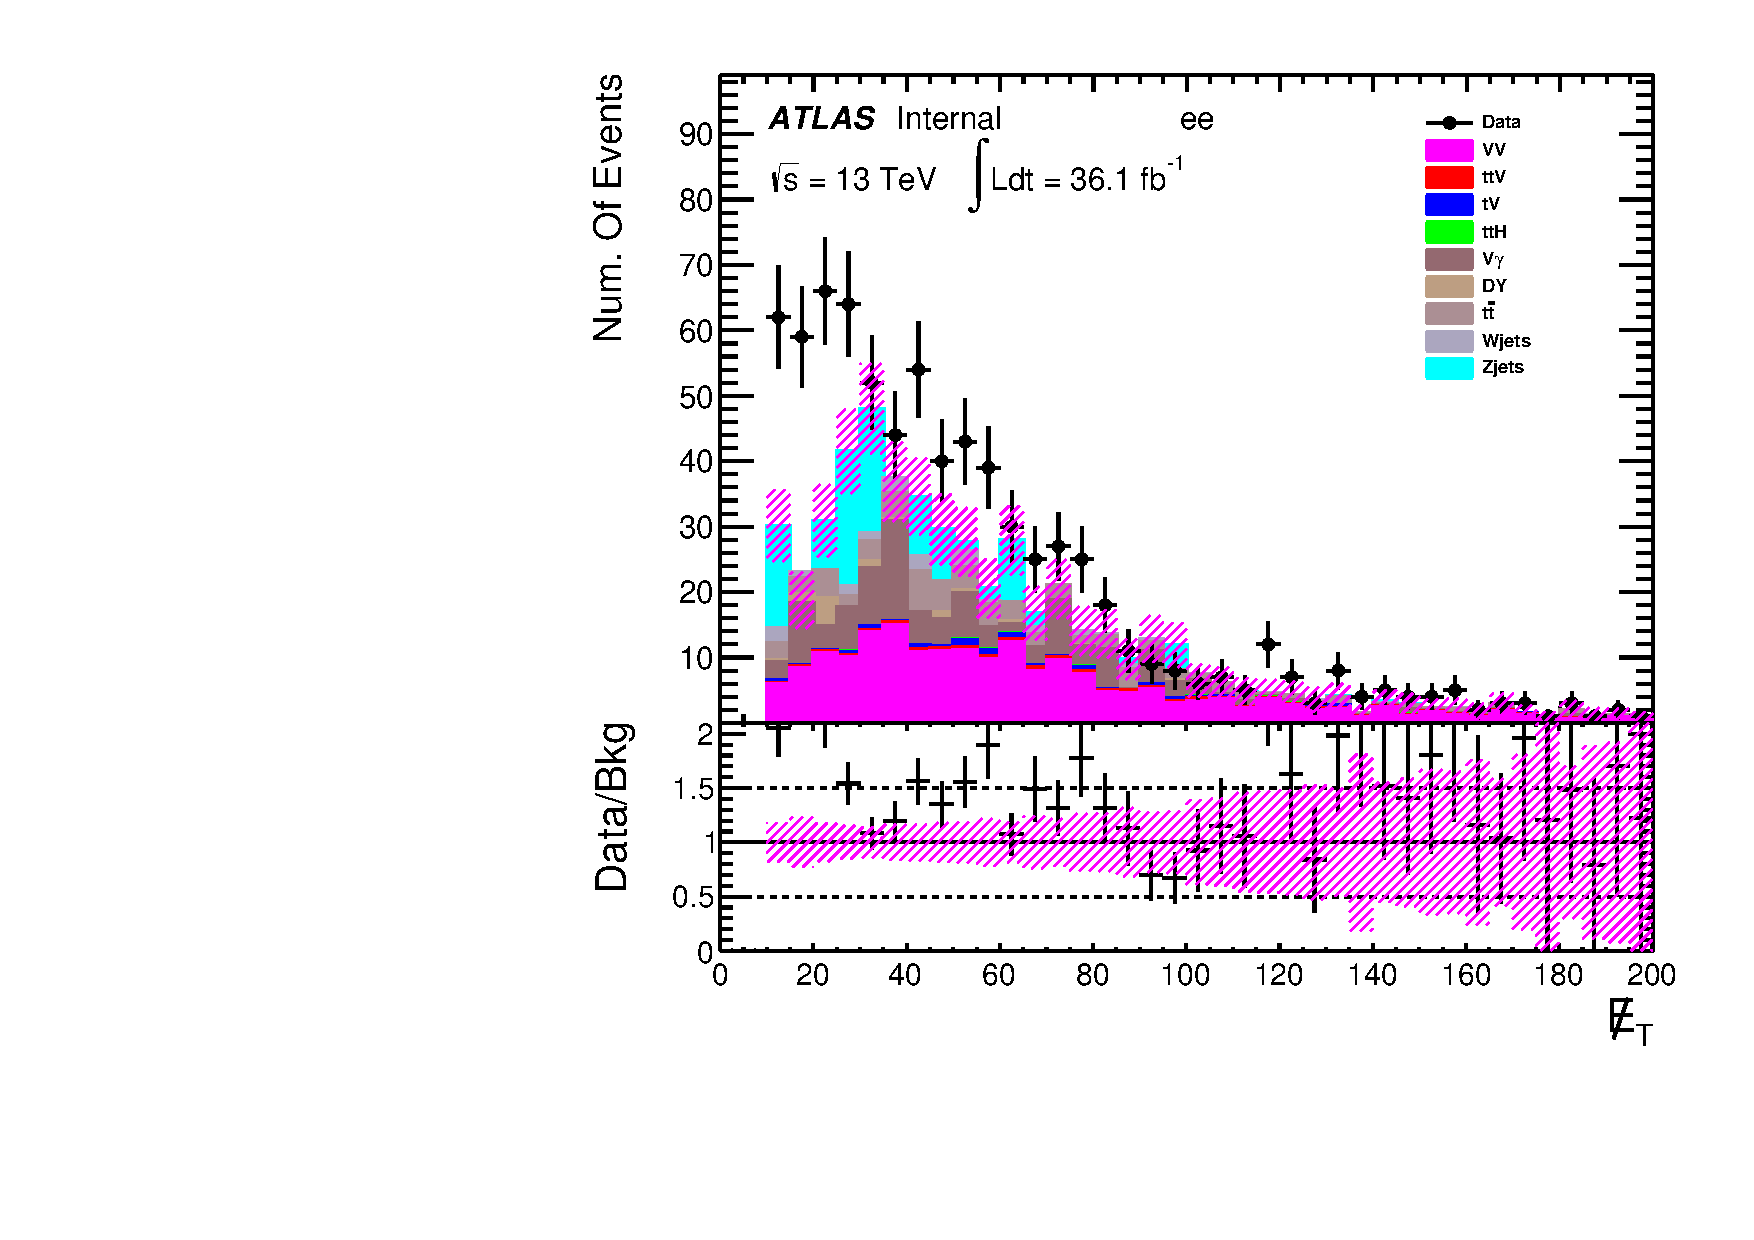
\includegraphics[width=1.0\textwidth,angle=-90]{fig/nominal/MET_ee.pdf}
 \label{fig:nominal:MET_ee.pdf}
 \end{minipage}
\begin{minipage}[t]{0.3\linewidth}
 \centering
 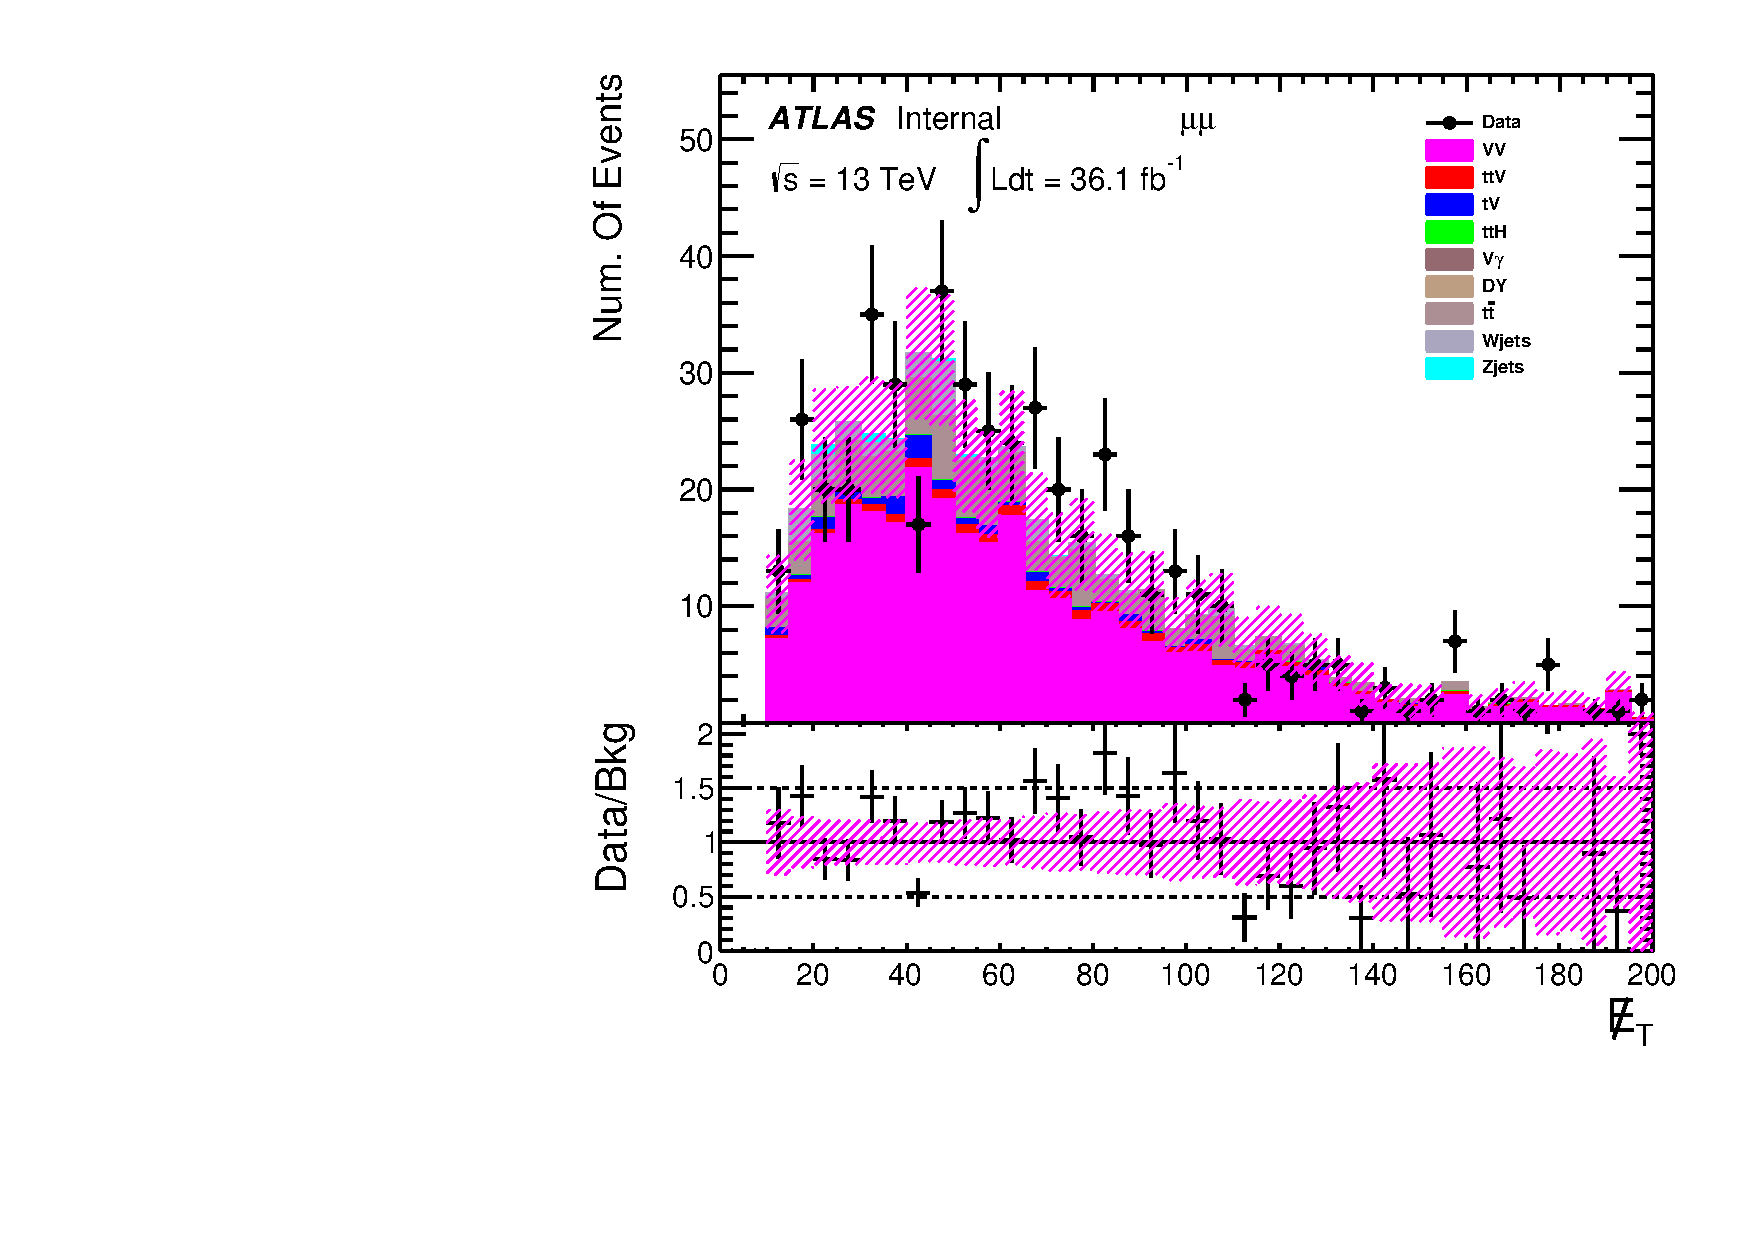
\includegraphics[width=1.0\textwidth,angle=-90]{fig/nominal/MET_mumu.pdf}
 \label{fig:nominal:MET_mumu.pdf}
 \end{minipage}
\begin{minipage}[t]{0.3\linewidth}
 \centering
 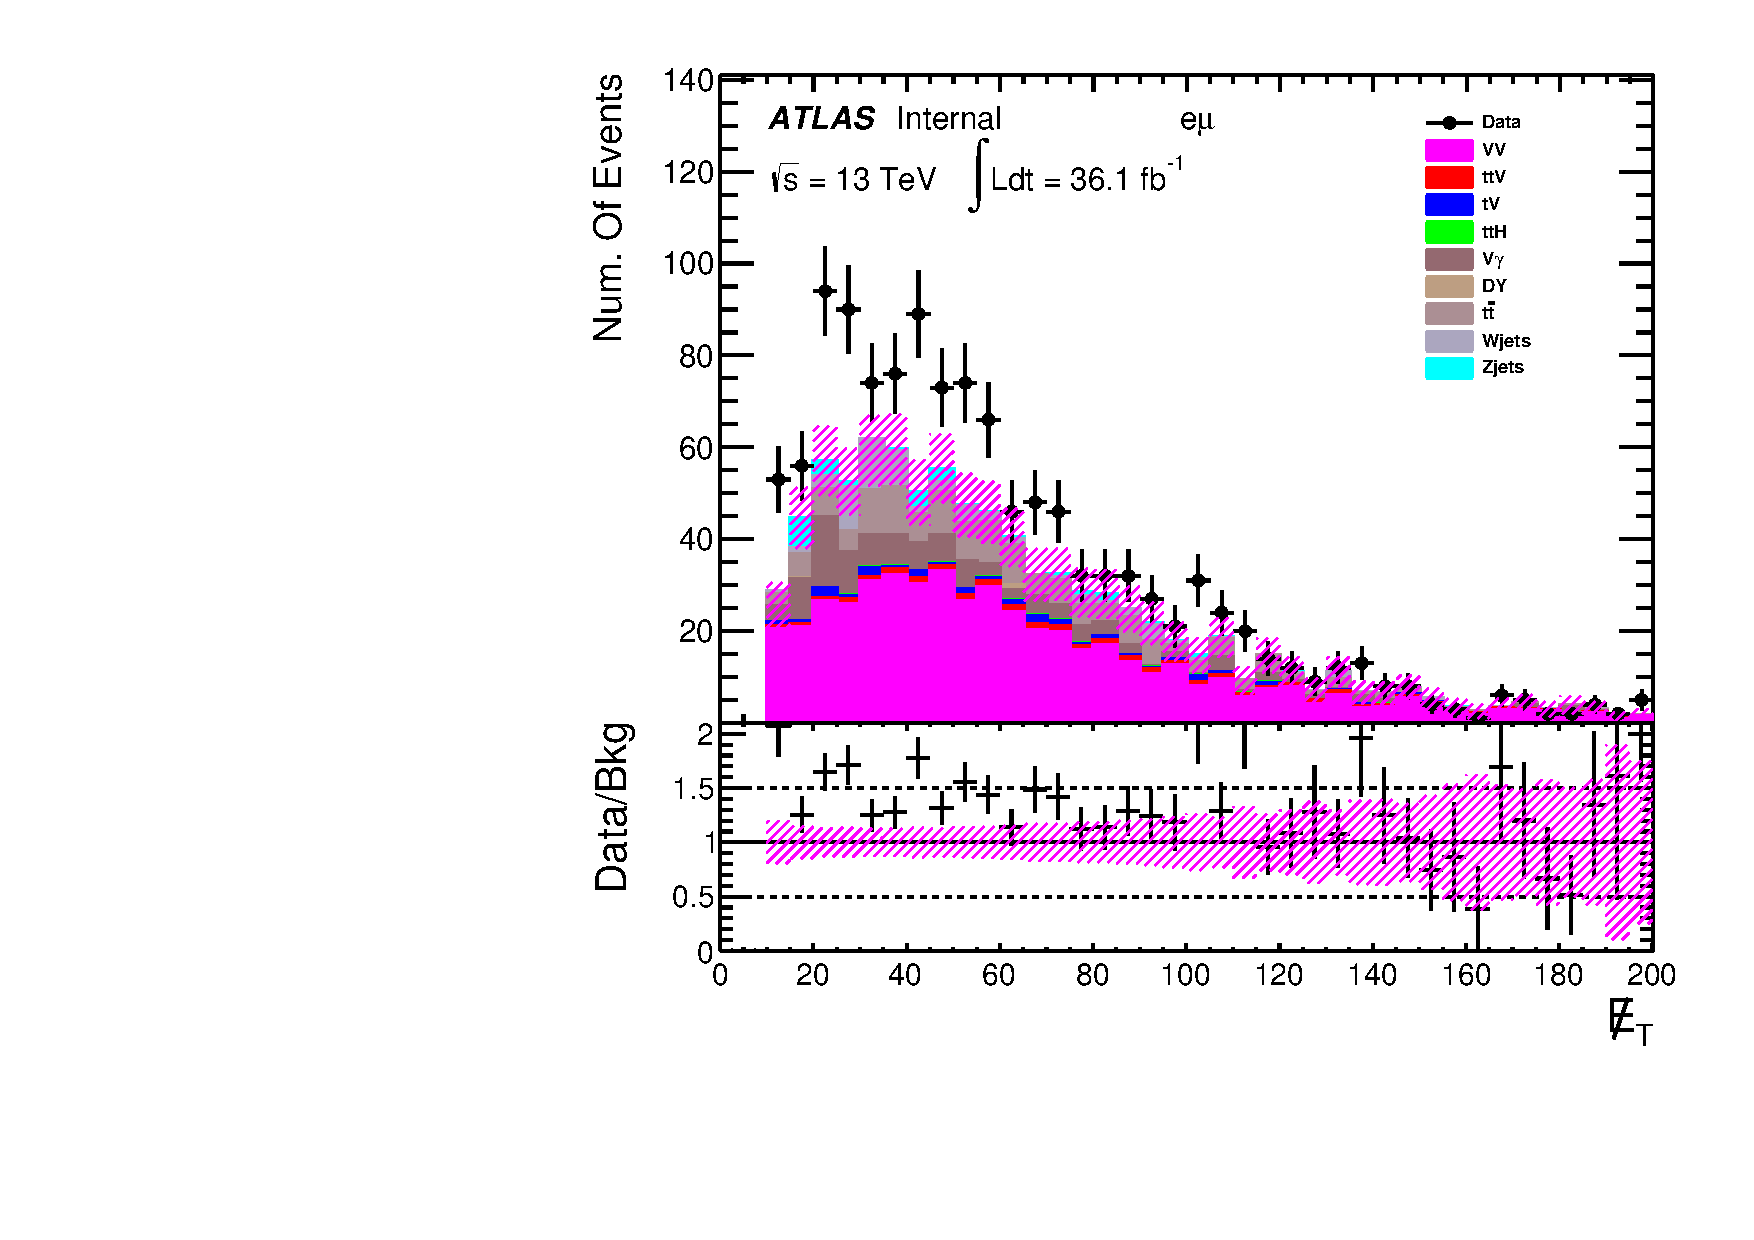
\includegraphics[width=1.0\textwidth,angle=-90]{fig/nominal/MET_emu.pdf}
 \label{fig:nominal:MET_emu.pdf}
 \end{minipage}
\begin{minipage}[t]{0.3\linewidth}
 \centering
 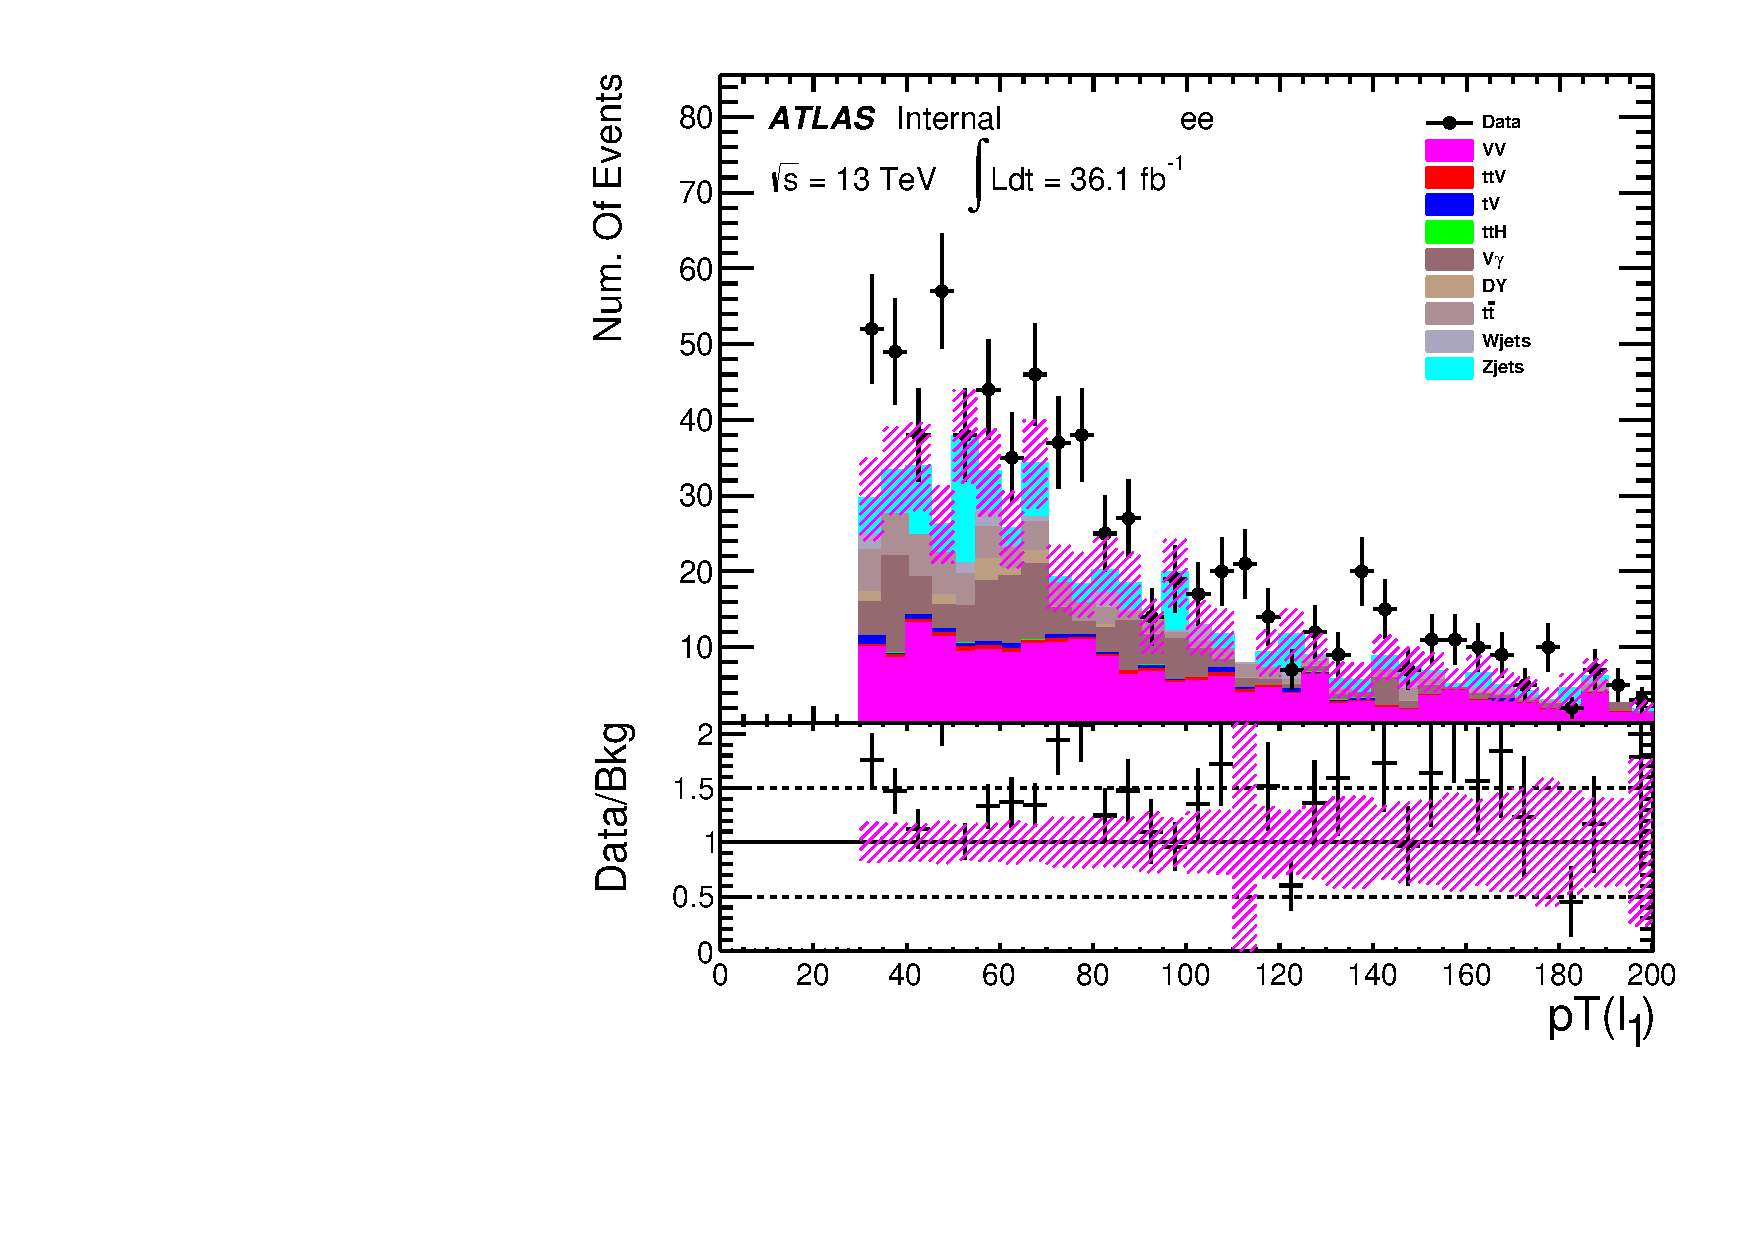
\includegraphics[width=1.0\textwidth,angle=-90]{fig/nominal/pt_leadinglepton_ee.pdf}
 \label{fig:nominal:pt_leadinglepton_ee.pdf}
 \end{minipage}
\begin{minipage}[t]{0.3\linewidth}
 \centering
 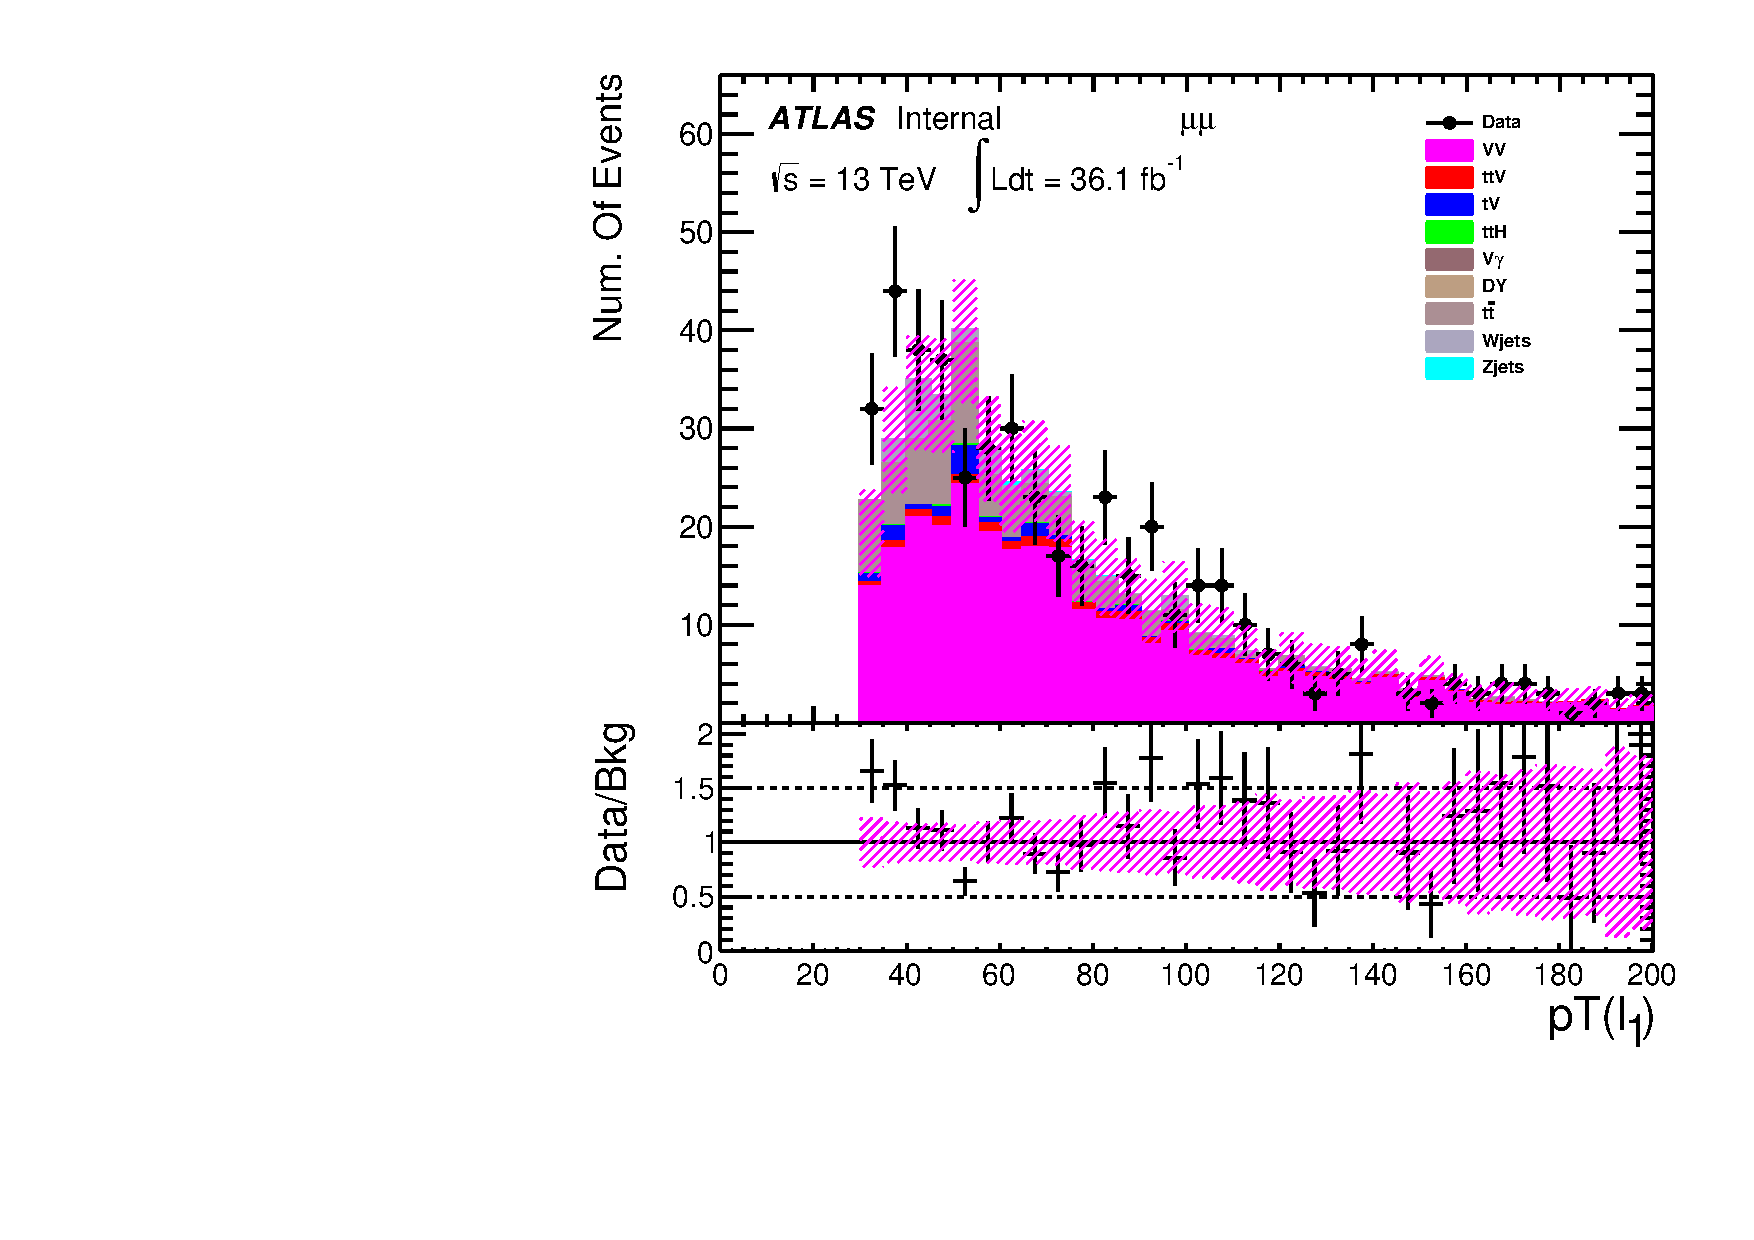
\includegraphics[width=1.0\textwidth,angle=-90]{fig/nominal/pt_leadinglepton_mumu.pdf}
 \label{fig:nominal:pt_leadinglepton_mumu.pdf}
 \end{minipage}
\begin{minipage}[t]{0.3\linewidth}
 \centering
 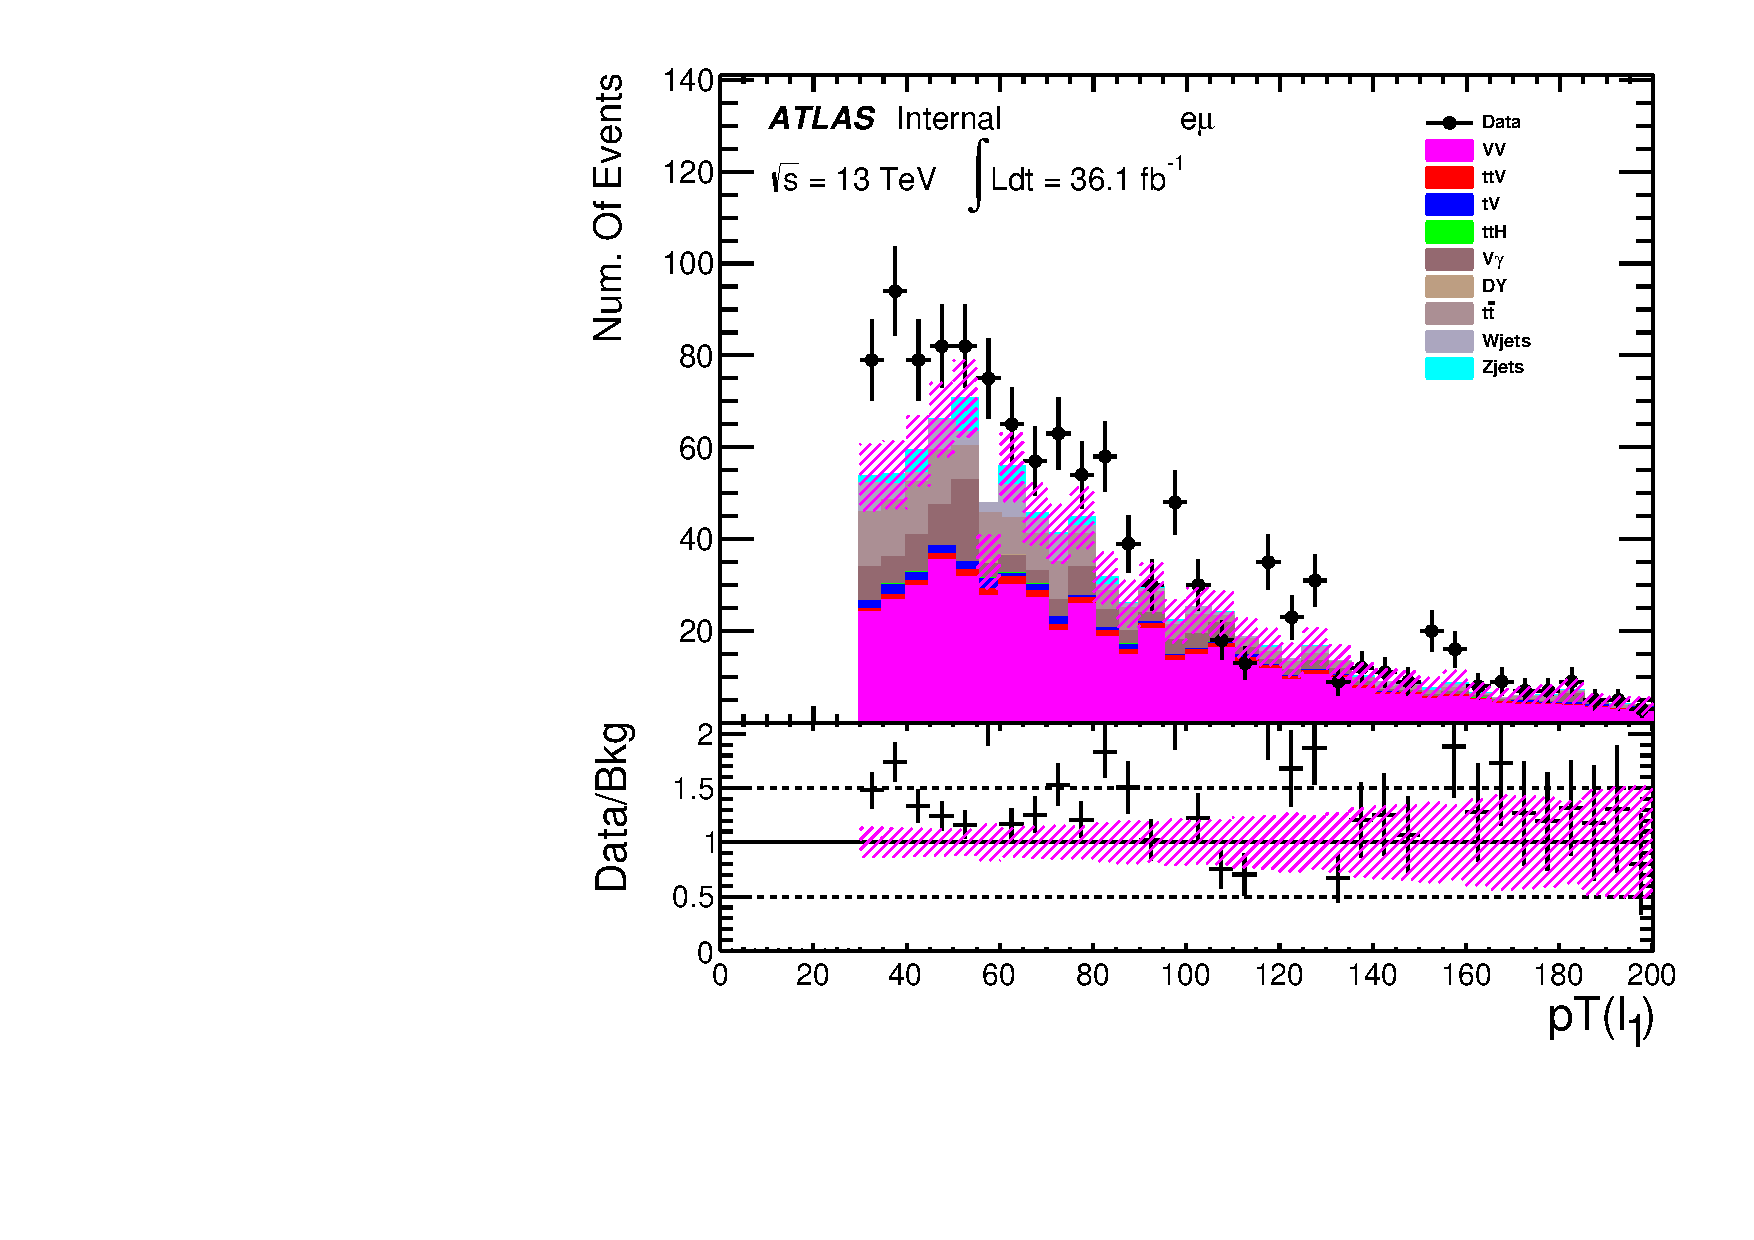
\includegraphics[width=1.0\textwidth,angle=-90]{fig/nominal/pt_leadinglepton_emu.pdf}
 \label{fig:nominal:pt_leadinglepton_emu.pdf}
 \end{minipage}
\begin{minipage}[t]{0.3\linewidth}
 \centering
 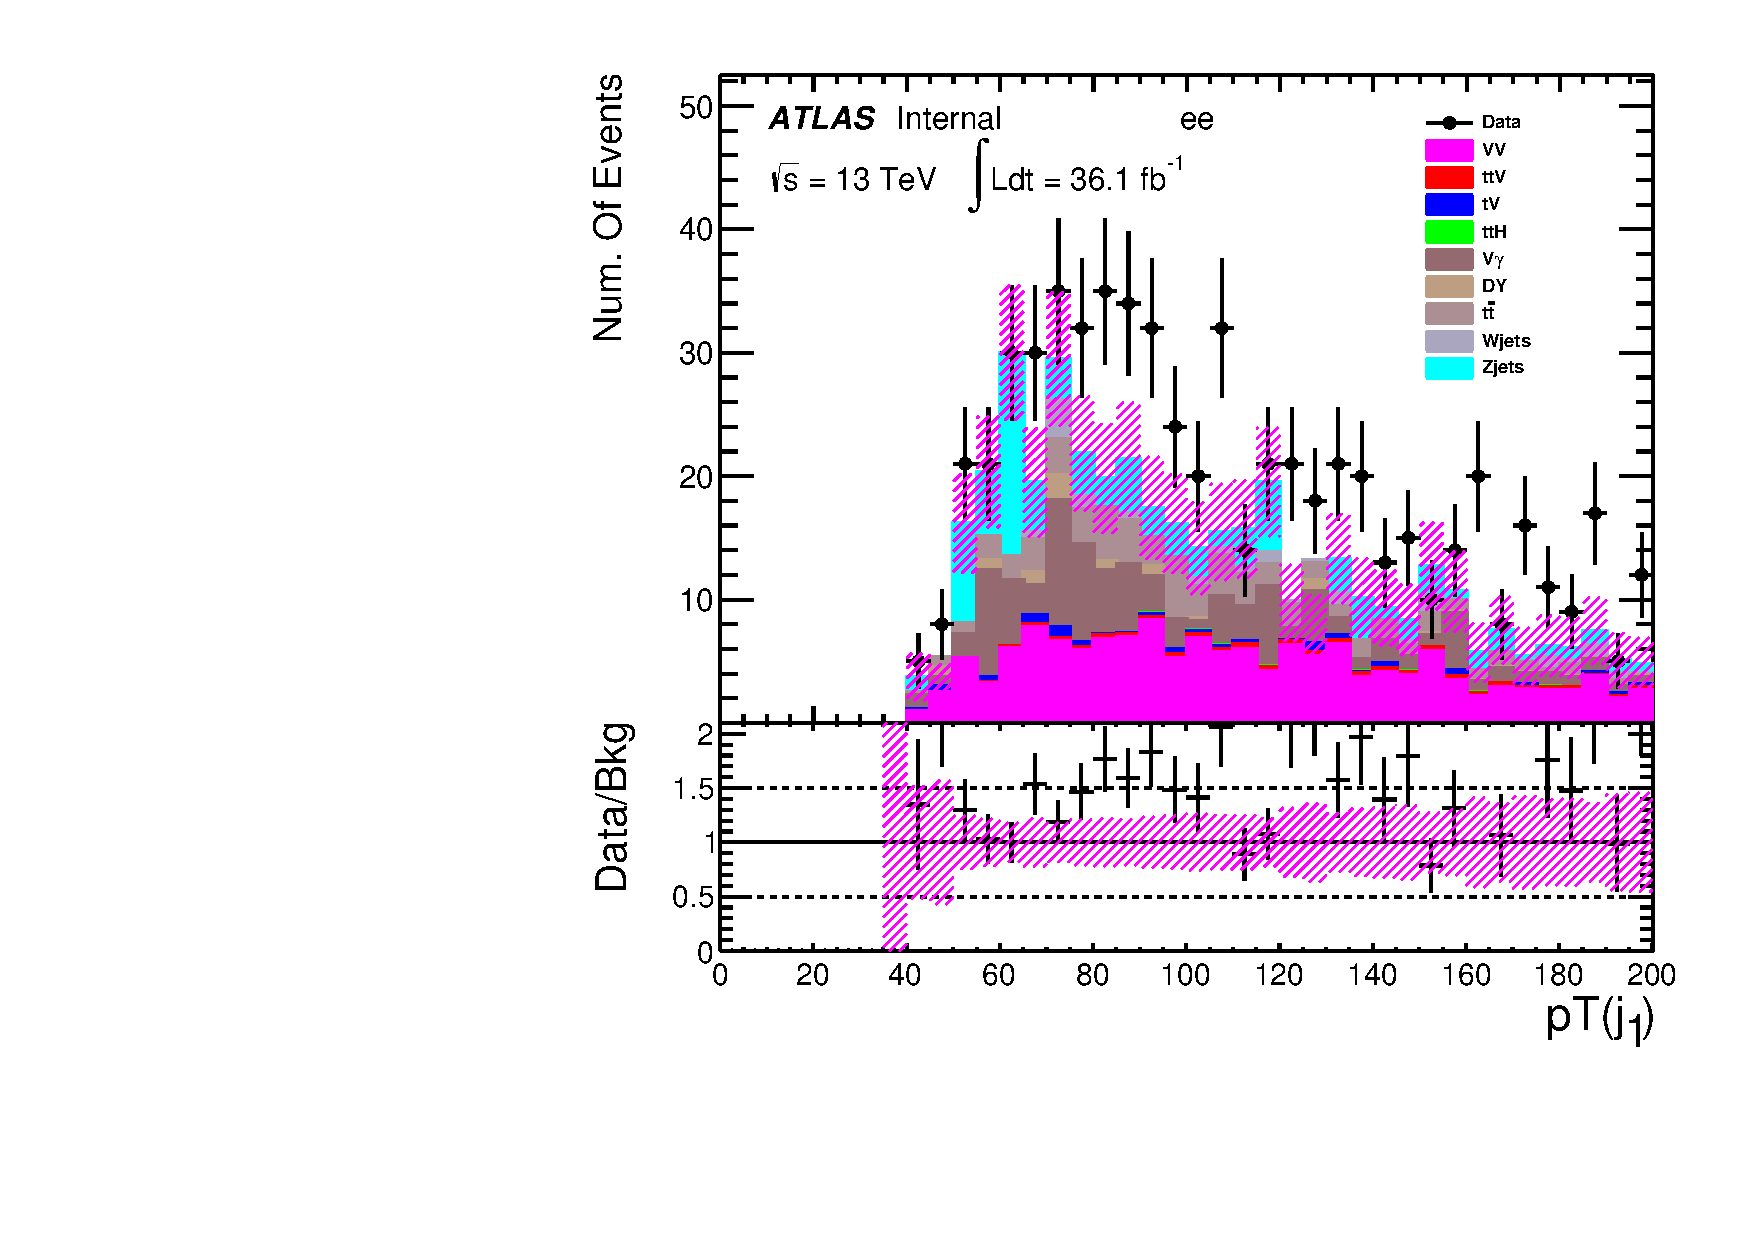
\includegraphics[width=1.0\textwidth,angle=-90]{fig/nominal/pt_j1_ee.pdf}
 \label{fig:nominal:pt_j1_ee.pdf}
 \end{minipage}
\begin{minipage}[t]{0.3\linewidth}
 \centering
 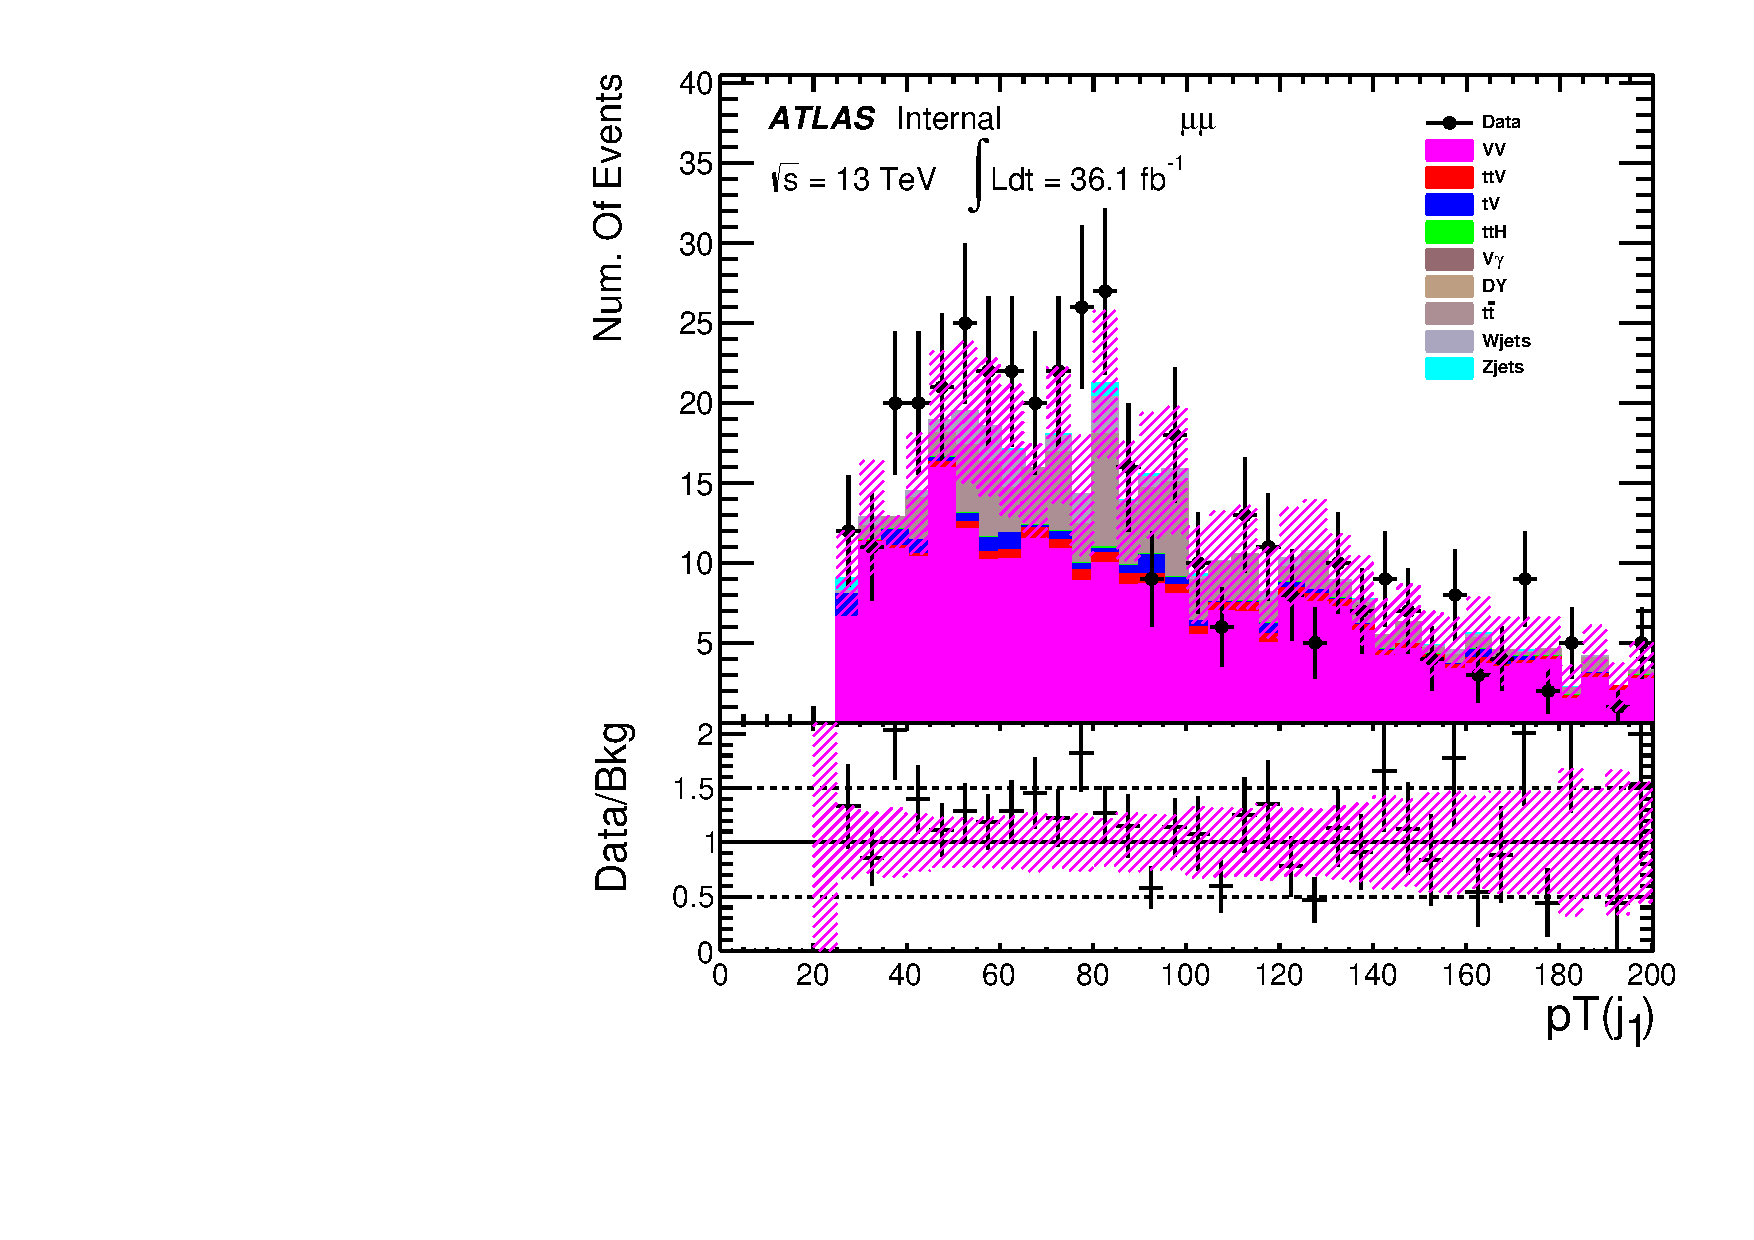
\includegraphics[width=1.0\textwidth,angle=-90]{fig/nominal/pt_j1_mumu.pdf}
 \label{fig:nominal:pt_j1_mumu.pdf}
 \end{minipage}
\begin{minipage}[t]{0.3\linewidth}
 \centering
 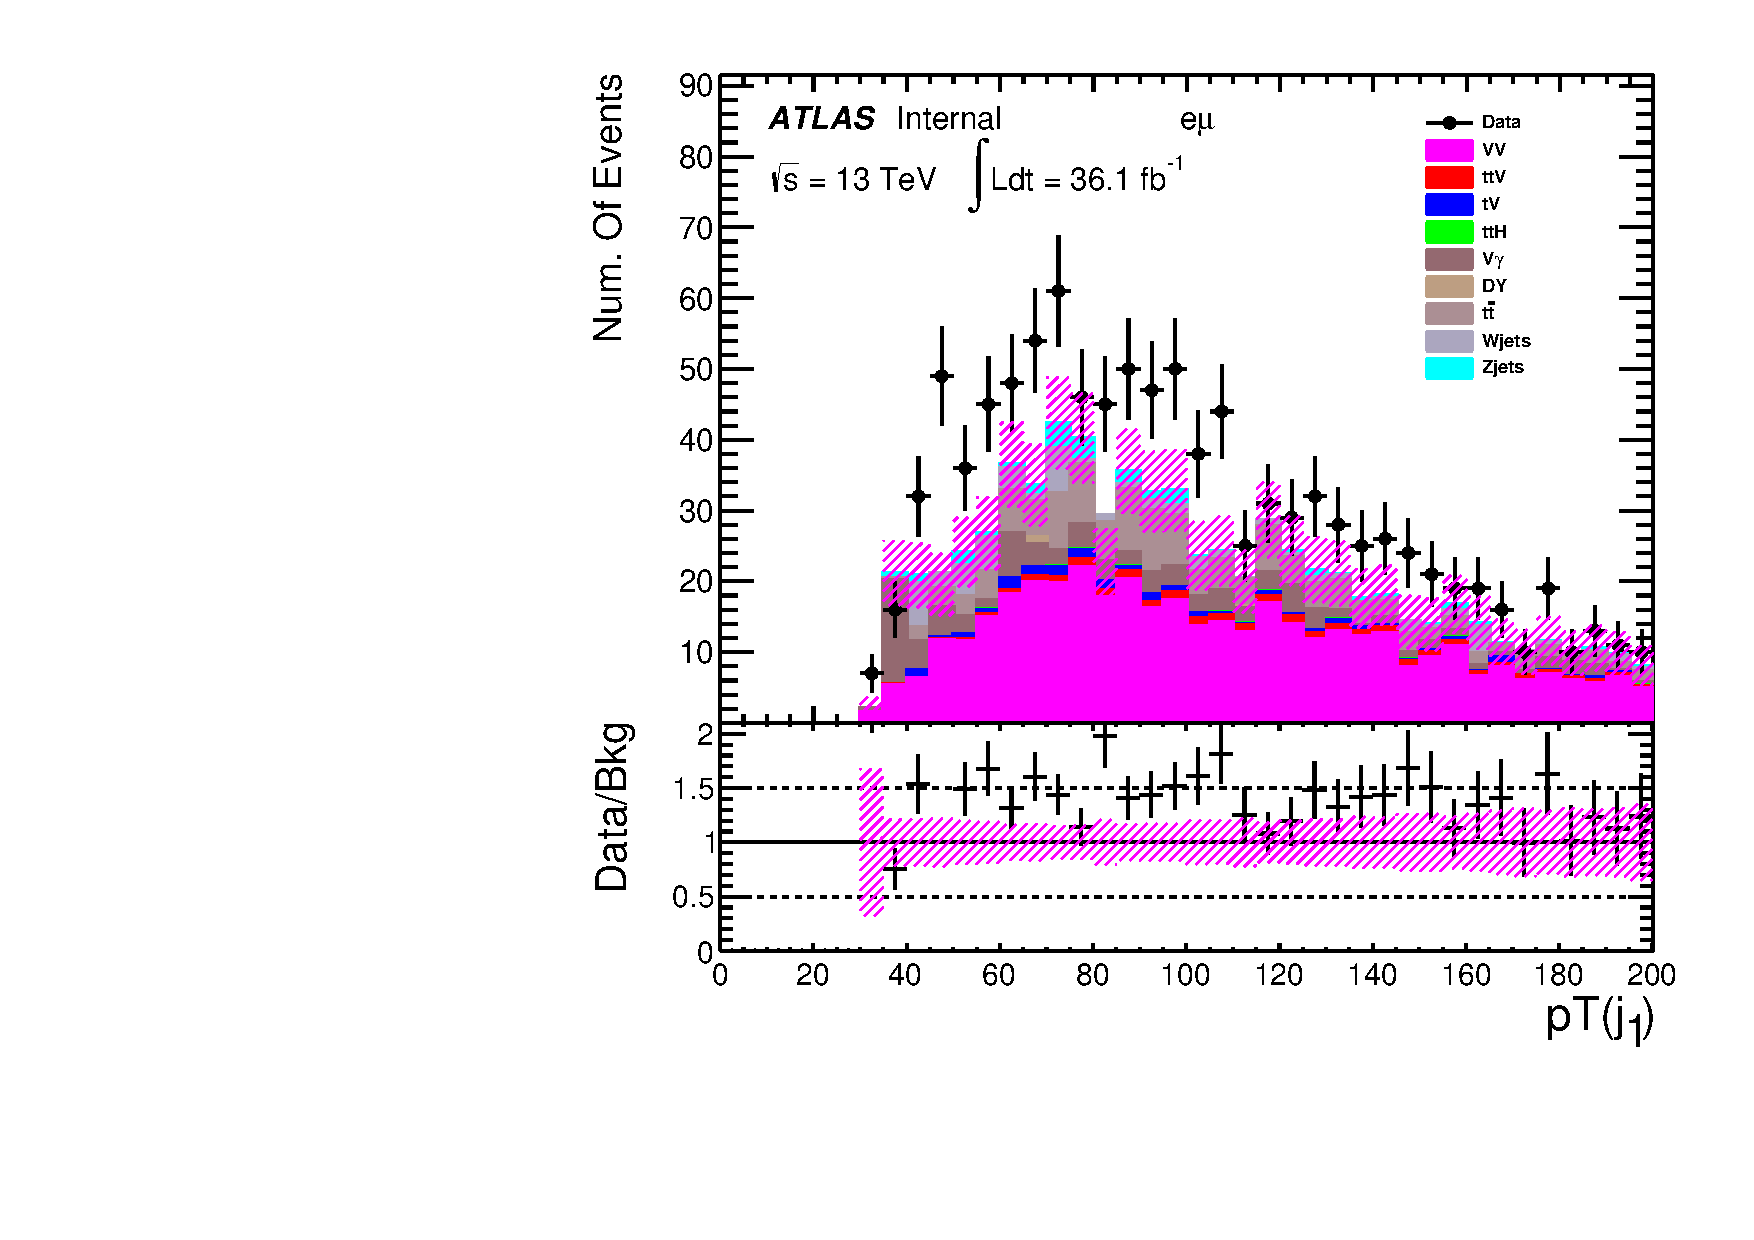
\includegraphics[width=1.0\textwidth,angle=-90]{fig/nominal/pt_j1_emu.pdf}
 \label{fig:nominal:pt_j1_emu.pdf}
 \end{minipage}
\caption{The comparison between data and all MC backgrounds at pre-selection level. Left: $ee$, middle: $\mu\mu$, right:$e\mu$. The slashed pink bands are corresponding to statistical uncertainties. Each process is normalized to the luminosity of 36.1 fb$^{-1}$.}
\label{fig:nominal:datavspureMC}
\end{figure}
\clearpage

\section{QmisID估计}\label{sec:QmisID_estimation}
双轻子为同电荷和同味道双轻子的$Z$ veto的选择条件,会极大地压低$t\bar{t}$和$Z+jets$背景,但如果一个电荷误判,即使很低的误判率,但考虑到这两种过程的极大截面,仍有相当一部分的QmisID会贡献到最终背景中。根据8 TeV的研究~\cite{MuonQmisIDnote},
$\mu$电荷误判率非常低(一般低于10$^{-5}$)
\footnote{The rate of charge mis-identification for muons is only affected by the track curvature. Because of the long lever arm to the muon system and the fact that the charge is measured in both the inner detector and muon spectrometer the mis-identification rates of the muon charge are very low, making this background negligible compared to the other sources of background},
所以只考虑电子电荷误判背景。\\
电子电荷误判有两种原因:
\begin{itemize}
  \item 当电子穿过探测器材料时,出射一个光子(韧致辐射);而后这个光子转换成一对正负电子,然而在随后的径迹重建中,带相反电荷的电子被利用,从而导致电荷误判。
韧致辐射依赖于探测器材料密度,而探测器材料密度随着\abseta 变化,所以电子的电荷误判率也依赖于\abseta。 
  \item 第二种贡献相对来讲比较小,主要是因为测量精度不够,当电子径迹的曲率很小或者内部探测器径迹与量能器的簇射匹配错误时,得到完全相反曲率的
径迹,从而导致电荷误判。所以,当电子具有高横动量时这个效应比较明显,那么误判率也依赖于\pt。
\end{itemize}
%\\
\subsection{似然函数方法}
一般假设电子电荷误判率不依赖于产生模式,因为$Z$玻色子产生截面大,而且其不变质量峰重建比较好,所以$Z$过程可以用来测量电子电荷误判率,采用似然函数技术~\cite{Likelihoodnote},构建的似然函数如下:
\begin{equation}
\ln L(\varepsilon|N_{SS},N)=\sum_{i,j}\ln [N^{ij}(\varepsilon_i+\varepsilon_j-2\varepsilon_i \varepsilon_j)]N^{ij}_{SS}-N^{ij}(\varepsilon_i+\varepsilon_j-2\varepsilon_i \varepsilon_j)
\end{equation}
其中,$\varepsilon_i$和$\varepsilon_j$分别为$\eta-\pt$二维区间中第i个和第j个电子的误判率,$N_{SS}$和$N$是观察到的
相同电荷事例数和总事例数。
$\eta-\pt$区域总共分为28个小区域,其$\abseta$和$\pt$的分界线分别为[0., 0.60, 1.1, 1.37, 1.52, 1.70, 2.00, 2.47]和
[10, 60, 90, 130, 1000] GeV。随后,为了得到电子电荷误判率,需按照以下过程进行:
\begin{enumerate}
 \item 按照$Z$玻色子过程筛选双轻子数据,其中轻子质量要求应与章节\ref{chap:evtsel}所述一致。
 \item 在所选数据中通过高斯函数拟合$Z$不变质量谱,得到$Z$不变质量拟合值$\kappa$和标准偏差$\sigma$。而后分为如下三个区间,
\begin{table}[h]
\centering
\begin{tabular}{cccc}
\hline
  A  &B  &C  \\
($\kappa-8\sigma$, $\kappa - 4\sigma$)  & ($\kappa \pm 4\sigma$)  & ($\kappa+4\sigma$, $\kappa + 8\sigma$) \\
\hline
\end{tabular}
\end{table}

 \item 为了进一步提高$Z$玻色子纯度,剩余本底会被减去,即$N_Z=n_B-\frac{n_A+n_C}{2}$。
 \item 所选数据根据电荷分为SS和OS,利用最大似然函数法得到各个$\abseta-\pt$区间的误判率。
\end{enumerate}
图\ref{fig:qmisid_rates}展示电子电荷误判率随着\abseta 增加而增大,因为在高\abseta 粒子会穿过更多探测器材料;误判率也随着\pt 增大而增大,这与前面的讨论一致。最后,利用公式~\ref{eq:qmisid_evts}计算出$ee$和$e\mu$道经过初步筛选后,在$N_{\text{jet}}\ge2$时($N_{\text{jet}}\ge3$)的误判事例数分别为101.47$\pm$0.60 (35.60$\pm$0.38)和18.21$\pm$0.23 (8.38$\pm$0.16)。
\begin{figure}[h]
 \centering
 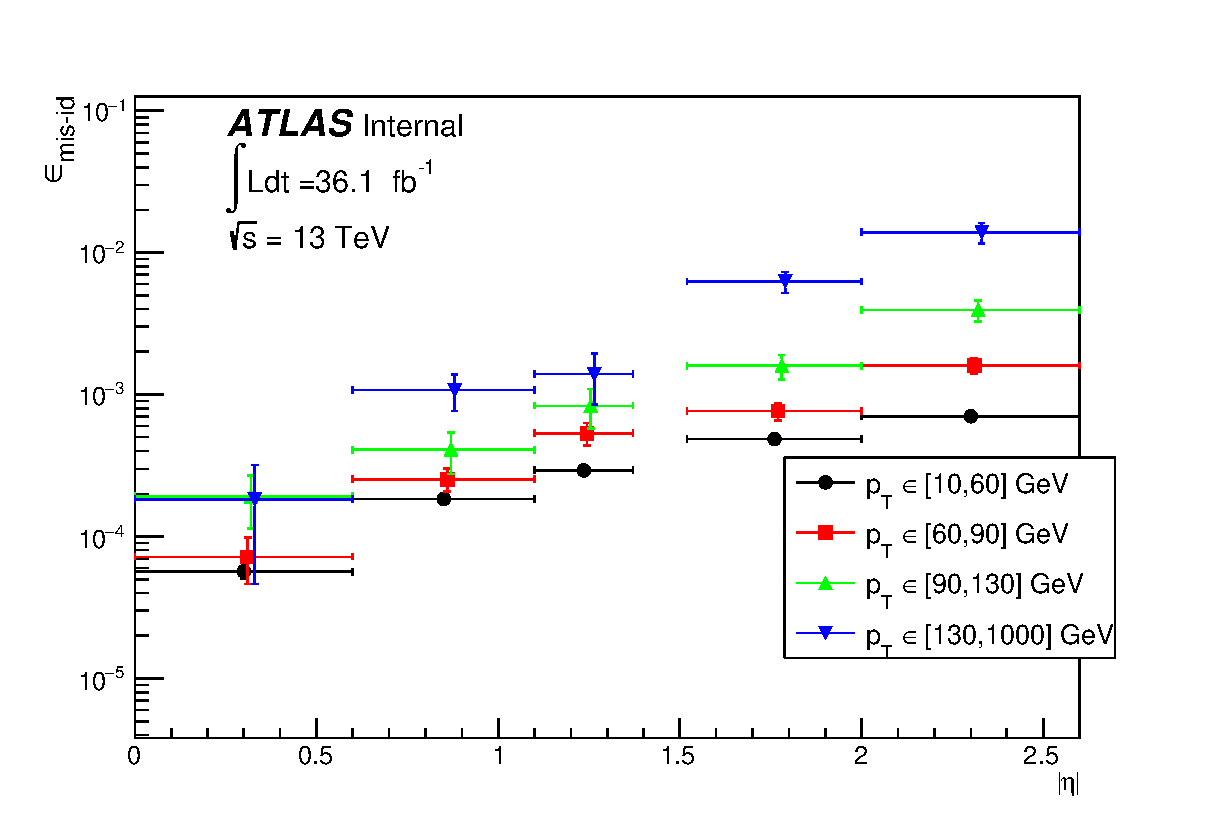
\includegraphics[width=0.70\textwidth]{fig/QmisID/Rates_tight.eps}
\caption{The electron charge mis-identification rates as a function of ($|\eta|$, $p_T$) computed in data with the likelihood method.}
\label{fig:qmisid_rates}
\end{figure}

\begin{equation}
N_{ee}^{\text{QmisID}}=\frac{\varepsilon_i+\varepsilon_j-2\varepsilon_i \varepsilon_j}{1-\varepsilon_i-\varepsilon_j +2\varepsilon_i \varepsilon_j}N^{\text{OS}},
N_{e\mu}^{\text{QmisID}}=\frac{\varepsilon}{1-\varepsilon}N^{\text{OS}}
\label{eq:qmisid_evts}
\end{equation}

\subsection{系统误差}
在QmisID估计中,考虑了三种系统误差:
\begin{enumerate}
 \item 每个$\abseta-\pt$ 小区域中的统计误差;
 \item 为了证实似然函数方法的可靠性,可以利用$Z$ MC进行以上的误判率估计,因为在MC中,电子误判率是已知的,从而比较似然函数
估计值与真实值就可判断该方法的可信程度(closure test)。图~\ref{fig:QmisID_TMLik}比较了真实值与似然函数估计值,总体上
是一致的。该项差距将作为QmisID的系统误差之一。
\begin{figure}[h]
\centering
 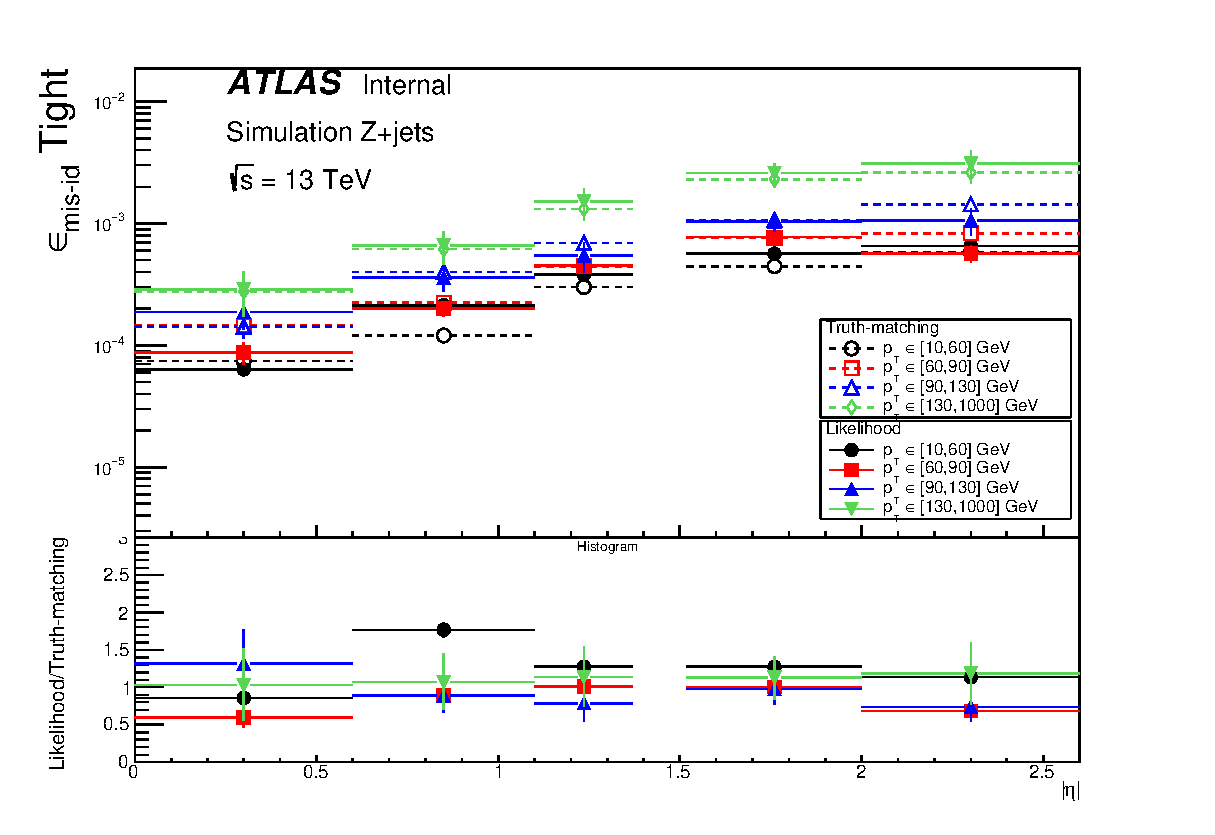
\includegraphics[width=0.70\textwidth]{fig/QmisID/TMLik_tight.eps}
 \caption{The comparison between the charge mis-identification rates of electrons measured in simulated $Z\rightarrow e^{+}e^{-}$ events with the truth-matching method and the 2D likelihood method.}
\label{fig:QmisID_TMLik}
\end{figure}

 \item $Z$峰区间的变动会影响QmisID的估计,所以,如果偏移$Z$峰1 $\sigma$,其QmisID 率的相对变化考虑成系统误差。
\end{enumerate}
图~\ref{fig:QmisID_syst}总结了几种系统误差在不同$\abseta-\pt$的相对大小,随着$\pt$的增加统计误差越来越大,因为
大部分电子是低动量的,其次是似然函数误差在低动量区更显著。
\begin{figure}[h]
\centering
  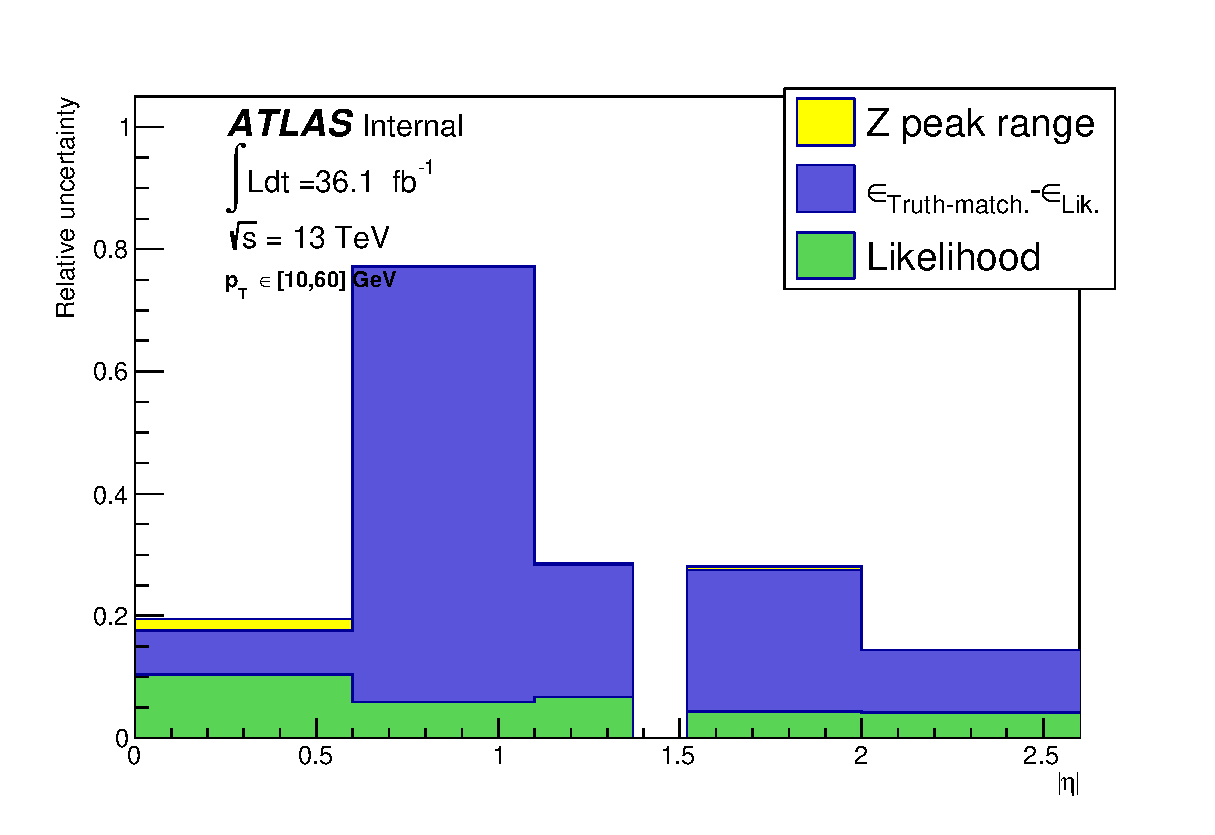
\includegraphics[width=0.45\textwidth]{fig/QmisID/Syst1_tight.eps}
  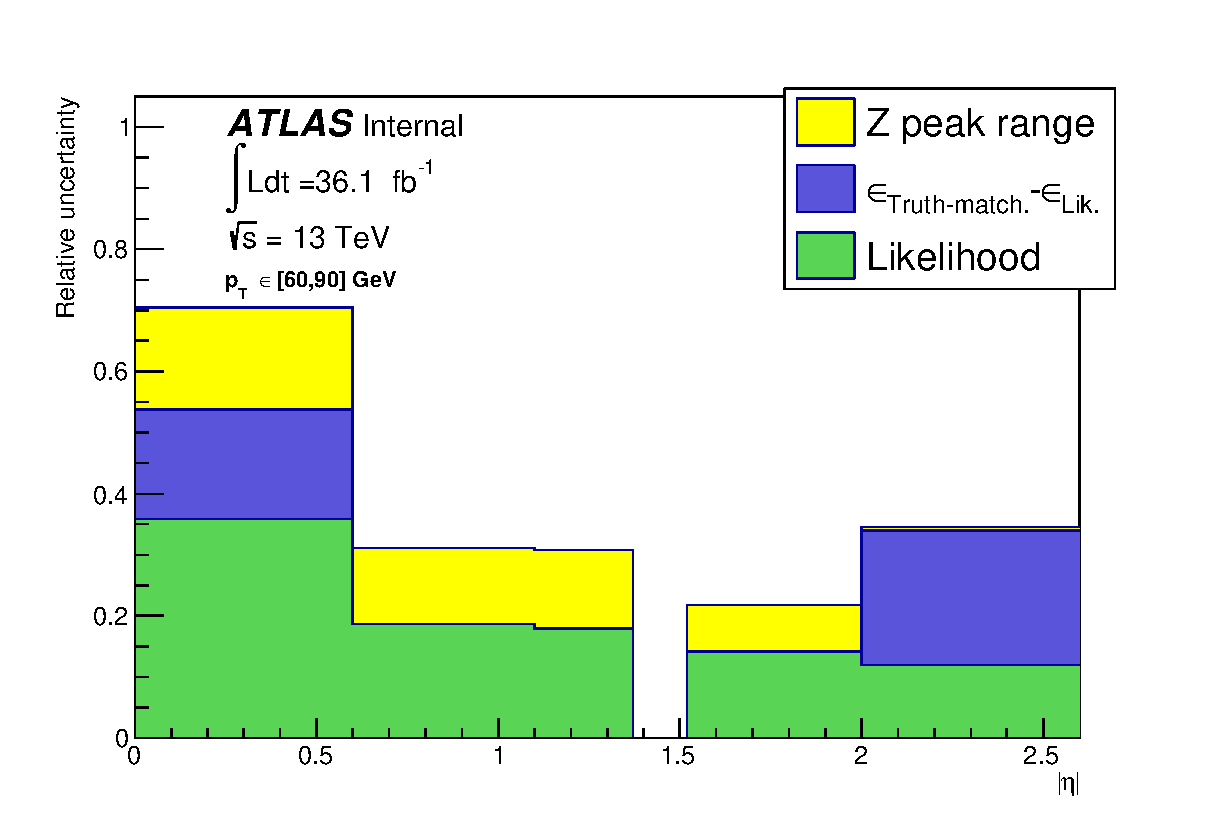
\includegraphics[width=0.45\textwidth]{fig/QmisID/Syst2_tight.eps}
  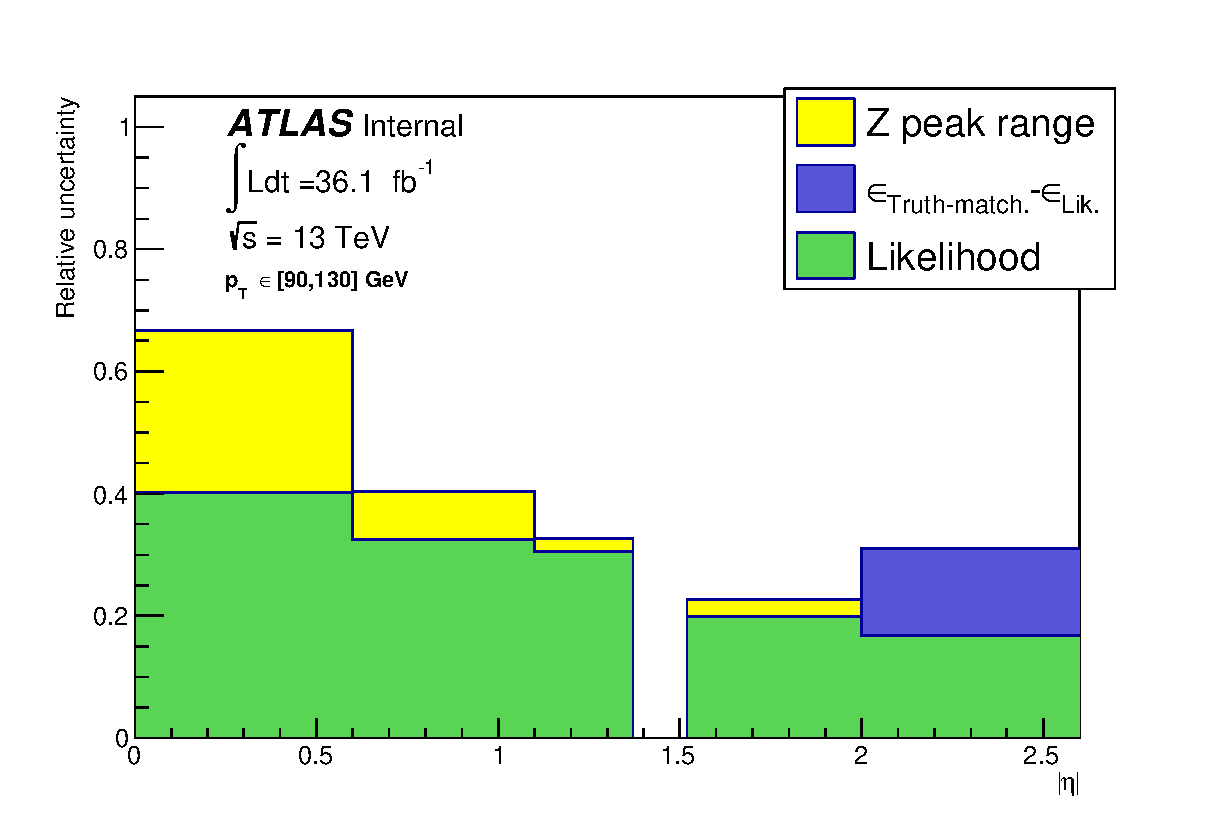
\includegraphics[width=0.45\textwidth]{fig/QmisID/Syst3_tight.eps}
  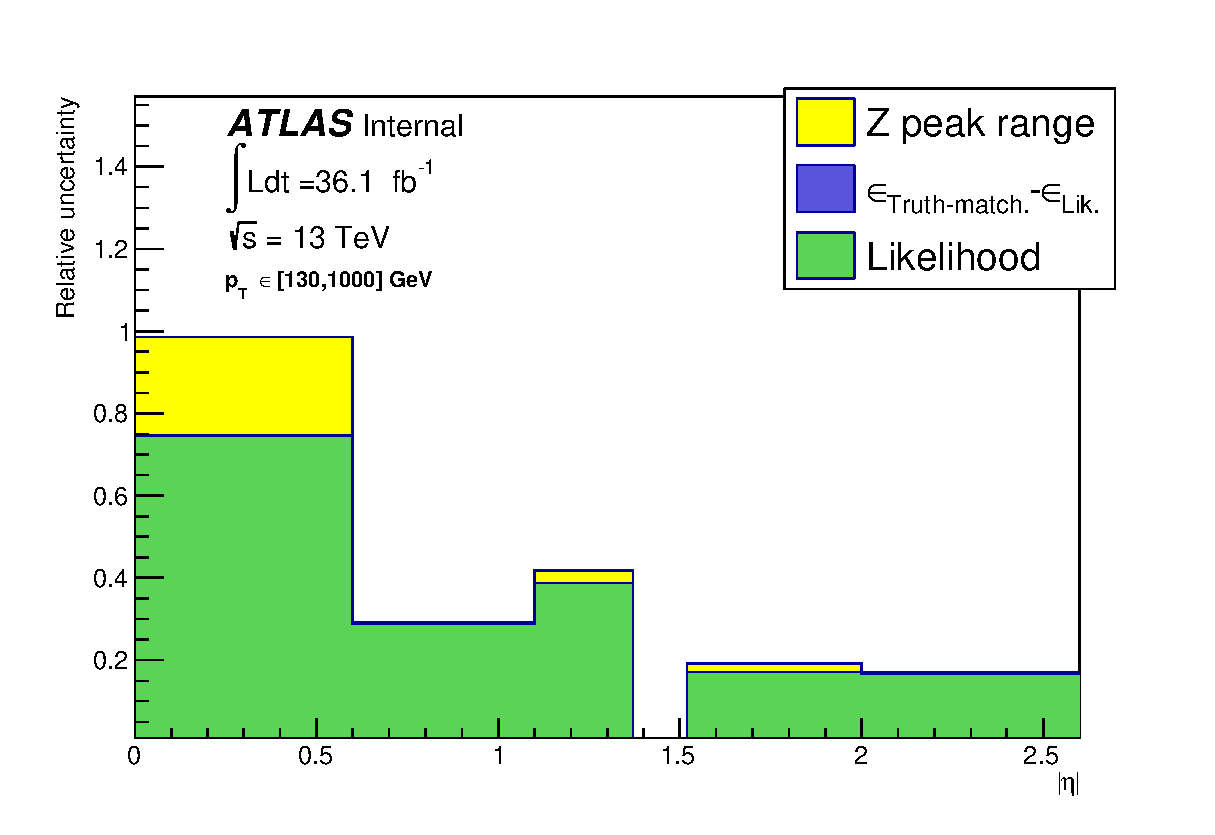
\includegraphics[width=0.45\textwidth]{fig/QmisID/Syst4_tight.eps}
\caption{The systematic uncertainty on the charge mis-identification rate, for different bins in $p_T$ and $|\eta|$.}
\label{fig:QmisID_syst}
\end{figure}

\section{Fakes估计}
误鉴别粒子是一项非常重要的本底,因为对其形成机制理解不够准确,MC并不能很好地描述,所以有必要使用data-driven的方法
去估计该项本底。在该分析中,我们使用fake factor的方法。

\subsection{Fake factor方法}
在4W分析中,Fake factor方法的假设是fake factor不依赖于jet数,其定义是具有两个\texttt{tight} SS轻子的事例数与具有
一个\texttt{tight}和一个\texttt{anti-tight}的轻子的事例数比例,如等式~\ref{eq:fake_factor_def}所示。
\begin{equation}
\theta_{\ell}=\frac{N_{\ell \ell}}{N_{\ell \cancel{\ell}}}
\label{eq:fake_factor_def}
\end{equation}
其中,$\ell$为\texttt{tight}电子或者$\mu$子,$\cancel{\ell}$是\texttt{anti-tight}的轻子。通常,分母的选择是fake 
factor中最困难的部分:分母的选择应当使得真实轻子极大地压低,而尽量增大误鉴别轻子的比例。如果分母选择条件越严格,
与外延相关的系统误差越小,但是另一方面,事例越少,相应的统计误差越大。所以,为了优化整体的系统误差,必须考虑到这
些相反的影响。一般来讲,利用ID和isolation条件可以很好地压低误鉴别的电子,而isolation和碰撞参数可以用来压低误鉴别
$\mu$子~\cite{Alison2015}。
在本分析中,$\ell$和$\cancel{\ell}$的定义如表~\ref{tab:tight_ele_def}和表~\ref{tab:tight_mu_def}所示。
\begin{table}[!ht]
\begin{center}
\begin{tabular}{c|cccccc}
\hline
  &tight electron    &anti-tight electron  \\
\hline
ID  &TightLH  &fail TightLH \\
isolation &isolationFixedCutTight  &- \\
QmisID          &ChargeIDBDTTight$>$0.067  &ChargeIDBDTTight$>$0.067 \\
\hline
\end{tabular}
\caption{definitions of tight electrons and anti-tight electrons. In addition to the inverted ID requirement, anti-tight
electrons are required to pass the loose selection criteria.}
\label{tab:tight_ele_def}
\end{center}
\end{table}

\begin{table}[!ht]
\begin{center}
\begin{tabular}{c|cccccc}
\hline
  &tight muon    &anti-tight muon  \\
\hline
ID  &Tight  &- \\
isolation &isolationFixedCutTightTrackOnly  &fail isolationFixedCutTightTrackOnly \\
\hline
\end{tabular}
\caption{definitions of tight muons and anti-tight muons. In addition to the inverted isolation requirement,
anti-tight muons are required to pass the loose selection criteria.}
\label{tab:tight_mu_def}
\end{center}
\end{table}
值得指出的是,因为在本分析中,有两个$N_{\text{jet}}$类别,所以对于低质量点,计算fake factor时要求一个jet;对于高质
量点,要求1到2个jet。总结如表~\ref{tab:summary_CRs_ff}所示。
\begin{table}[!ht]
\begin{center}
\scriptsize
\begin{tabular}{cc|c|c}
\hline
\multicolumn{2}{c|}{Region}  &Fake factor CR (low jet multilicity region) &SR (high jet multiplicity region)  \\
\hline
\multirow{2}{*}{Low mass} &$hh$: $m_X$=260, 300 GeV  &$N_{\text{jet}}$=1    &$N_{\text{jet}} \geq$2 \\
                          &$SS$: Fixing $m_S$=135 GeV, $m_X$=280, 300, 320 GeV  &  & \\
\hline
\multirow{2}{*}{High mass} &$hh$: $m_X$=400, 500 GeV, no-resonant  &$1\leq N_{\text{jet}} \leq 2$    &$N_{\text{jet}} \geq$3 \\
                          &$SS$: Fixing $m_X$=340 GeV, $m_S$=135, 145, 155 and 165 GeV  &  & \\

\hline
\end{tabular}
\caption{Summary of different regions used to estimate fakes for low mass and high mass searches.}
\label{tab:summary_CRs_ff}
\end{center}
\end{table}
接下来,作为例子,我们将只展示高质量点的fakes的计算方式。之前提过,本底包括fakes, QmisID, $V\gamma$和promptSS,
为了不重复考虑这些本底,实际计算fake factor时应当减去这些本底,如公式~\ref{eq:fake_factor_cal}所示。
\begin{equation}
\theta_{e}(1\leq N_{\text{jet}}\leq 2)=\frac{N_{ee}^{\text{data}}-N_{ee}^{\text{promptSS}}-N_{ee}^{V\gamma}-N_{ee}^{\text{QmisID}}}{N_{e\cancel{e}}^{\text{data}}-N_{e\cancel{e}}^{\text{promptSS}}-N_{e\cancel{e}}^{V\gamma}-N_{e\cancel{e}}^{\text{QmisID MC}}}(1\leq N_{\text{jet}}\leq 2)
\end{equation}
\begin{equation}
\theta_{\mu}(1\leq N_{\text{jet}}\leq 2)=\frac{N_{\mu\mu}^{\text{data}}-N_{\mu\mu}^{\text{promptSS}}-N_{\mu\mu}^{V\gamma}}{N_{\mu\cancel{\mu}}^{\text{data}}-N_{\mu\cancel{\mu}}^{\text{promptSS}}-N_{\mu\cancel{\mu}}^{V\gamma}}(1\leq N_{\text{jet}}\leq 2)
\label{eq:fake_factor_cal}
\end{equation}
可以看到,promptSS,QmisID和$V\gamma$在分子分母中均被减去。
promptSS用MC估计,并且要求其中一个轻子能够匹配到真实轻子(truth-matching)。$V\gamma$也利用MC估计,但是并不要求
truth-matching,因为其中一个轻子很可能来自于$\gamma$。对于QmisID,分子中的$N_{ee}^{\text{QmisID}}$计算如章节~\ref{sec:QmisID_estimation}所述,而$N_{e\cancel{e}}^{\text{QmisID MC}}$直接利用MC估计,其中要求电子truth-matching。表
~\ref{tab:ff_ele_CR_1jets}到表~\ref{tab:ff_mu_CR_2jets}总结在不同$N_{\text{jet}}$类别下,用来计算fake factor各个成分的值。
\begin{table}[!ht]
\begin{center}
\small
\begin{tabular}{c|c|cccc|c|c|c}
\hline
\hline
\multicolumn{2}{c|}{ Selections} &$VV$  &$t\bar{t}V$    &$tV$    &$t\bar{t}H$     &$V\gamma$  &QmisID  &Data \\
\hline
\multirow{2}{*}{$N_\text{jet}$ ==1}  &$ee$  &204.64$\pm$19.13 &1.09$\pm$0.08&5.08$\pm$0.93&0.03$\pm$0.01&135.94$\pm$12.84&164.46$\pm$0.65 &976\\
\cline{2-9}
                &$e\cancel{e}$ &44.26$\pm$3.51    &0.13$\pm$0.03  &8.25$\pm$1.32 &0.00$\pm$0.00  &67.33$\pm$10.49  &135.54$\pm$71.62    &1116\\
\hline
\hline
\end{tabular}
\caption{Observed number of data and expected events yields in low jet multiplicity region, which is used for fake factor calculation of electron in low mass search. Uncertainties are statistical.}
\end{center}
\end{table}

\begin{table}[!ht]
\begin{center}
\small
\begin{tabular}{c|c|cccc|c|c}
\hline
\hline
\multicolumn{2}{c|}{ Selections} &$VV$  &$t\bar{t}V$    &$tV$    &$t\bar{t}H$     &$V\gamma$    &Data \\
\hline
\multirow{2}{*}{$N_\text{jet}$ ==1}  &$\mu\mu$ &296.37$\pm$9.72    &1.92$\pm$0.11    &5.91$\pm$1.01    &0.02$\pm$0.02    &0.00$\pm$0.00 &455\\
\cline{2-8}
                  &$\mu\cancel{\mu}$ &56.84$\pm$5.00    &0.13$\pm$0.03    &20.80$\pm$2.34    &0.00$\pm$0.00    &0.63$\pm$0.45    &378\\
\hline
\hline
\end{tabular}
\caption{Observed number of data and expected events yields in low jet multiplicity region, which is used for fake factor calculation of muon in low mass search. Uncertainties are statistical.}
\end{center}
\end{table}


\begin{table}[!ht]
\begin{center}
\scriptsize
\begin{tabular}{c|c|cccc|c|c|c}
\hline
\hline
\multicolumn{2}{c|}{ Selections}                      &$VV$  &$t\bar{t}V$    &$tV$    &$t\bar{t}H$     &$V\gamma$  &QmisID  &Data \\
\hline
\multirow{2}{*}{$1\leq N_{\text{jet}} \leq 2$}  &$ee$ &309.38$\pm$19.75    &3.67$\pm$0.16    &11.27$\pm$1.47    &0.10$\pm$0.02    &213.30$\pm$17.29    &230.40$\pm$0.81    &1434 \\
\cline{2-9}                                       &$e\cancel{e}$ &66.58$\pm$5.19    &0.39$\pm$0.06    &15.85$\pm$1.89    &0.02$\pm$0.01    &104.00$\pm$12.71    &187.16$\pm$78.65    &1591 \\
\hline
\hline
\end{tabular}
\caption{电子Fake factor CR ($1\leq N_{\text{jet}} \leq 2$)中的数据与预期本底数,不确定度仅是统计误差。}
%\caption{Observed number of data and expected events yields in low jet multiplicity region, which is used for fake factor calculation of electron in high mass search. Uncertainties are statistical.}
\end{center}
\end{table}

\begin{table}[!ht]
\centering
\scriptsize
\begin{tabular}{c|c|cccc|c|c}
\hline
\hline
\multicolumn{2}{c|}{ Selections}                           &$VV$  &$t\bar{t}V$    &$tV$    &$t\bar{t}H$     &$V\gamma$    &Data \\
\hline
\multirow{2}{*}{$1\leq N_{\text{jet}} \leq 2$}   &$\mu\mu$ &463.01$\pm$11.61    &6.14$\pm$0.21    &15.20$\pm$2.26    &0.17$\pm$0.03    &0.01$\pm$0.01    &729 \\
\cline{2-8}
                                        &$\mu\cancel{\mu}$ &74.30$\pm$5.40    &0.45$\pm$0.06    &43.59$\pm$3.37    &0.02$\pm$0.01    &1.62$\pm$0.74    &658 \\
\hline
\hline
\end{tabular}
\caption{$\mu$子Fake factor CR ($1\leq N_{\text{jet}} \leq 2$)中的数据与预期本底数,不确定度仅是统计误差。}
%\caption{Observed number of data and expected events yields in low jet multiplicity region, which is used for fake factor calculation of muon in high mass search. Uncertainties are statistical.}
\label{tab:ff_mu_CR_2jets}
\end{table}

最终,根据公式~\ref{eq:fake_factor_cal},得到各种类别的fake factor,总结在表~\ref{tab:summary_fake_factor}。
\begin{table}[!ht]
\begin{center}
\begin{tabular}{c|c|c}
\hline
\hline
Selections  &Fake factor   &Value  \\
\hline
\multirow{2}{*}{$N_\text{jet}$ ==1} &$\theta_{e}$   &0.5401$\pm$0.0311    \\
\cline{2-3}
                                    &$\theta_{\mu}$ &0.5033$\pm$0.0503    \\
\hline
\multirow{2}{*}{$1\leq N_{\text{jet}} \leq 2$}  &$\theta_{e}$   &0.5472$\pm$0.0264    \\
\cline{2-3}
                                                &$\theta_{\mu}$ &0.4544$\pm$0.0350    \\
\hline
\hline
\end{tabular}
\caption{Summary of fake factors of electron and muon with different $N_{\text{jet}}$ requirements. Uncertainties are statistical.}
\label{tab:summary_fake_factor}
\end{center}
\end{table}

接下来,就可以计算在信号区,即高$N_{text{jet}}$区,的fakes估计值。计算方法如下:
\begin{equation}
N_{ee}^{\text{fakes}}(N_{\text{jet}}\geq 3)=(N_{e\cancel{e}}^{\text{data}}-N_{e\cancel{e}}^{\text{promptSS}}-N_{e\cancel{e}}^{V\gamma}-N_{e\cancel{e}}^{\text{QmisID MC}})(N_{\text{jet}}\geq 3)\times \theta_{e}
\end{equation}
\begin{equation}
N_{\mu\mu}^{\text{fakes}}(N_{\text{jet}}\geq 3)=(N_{\mu\cancel{\mu}}^{\text{data}}-N_{\mu\cancel{\mu}}^{\text{promptSS}}-N_{\mu\cancel{\mu}}^{V\gamma})(N_{\text{jet}}\geq 3)\times \theta_{\mu}
\end{equation}
\begin{equation}
\begin{split}
N_{e\mu}^{\text{fakes}}(N_{\text{jet}}\geq 3)=(N_{e\cancel{\mu}}-N_{e\cancel{\mu}}^{\text{promptSS}}-N_{e\cancel{\mu}}^{V\gamma}-N_{e\cancel{\mu}}^{\text{QmisID}})(N_{\text{jet}}\geq 3)\times \theta_{\mu} \\ +
       (N_{\cancel{e}\mu}-N_{\cancel{e}\mu}^{\text{promptSS}}-N_{\cancel{e}\mu}^{V\gamma}-N_{\cancel{e}\mu}^{\text{QmisID MC}})(N_{\text{jet}}\geq 3)\times \theta_{e}
\end{split}
\end{equation}
各个成分的选择同样遵循计算fake factor时要求,表~\ref{tab:low_Njet_CR_eventyield}(表~\ref{tab:high_Njet_CR_eventyield})总结各种成分在$N_{text{jet}}\ge2$($N_{text{jet}}\ge3$)时的数值。
\begin{table}[!ht]
\begin{center}
\small
\begin{tabular}{c|c|cccc|c|c|c}
\hline
\hline
\multicolumn{2}{c|}{ Selections}                      &$VV$  &$t\bar{t}V$    &$tV$    &$t\bar{t}H$     &$V\gamma$  &QmisID  &Data \\
\hline
\multirow{2}{*}{$N_{\text{jet}} \geq 2$}  &$e\cancel{e}$ &37.39$\pm$4.24  &1.67 $\pm$ 0.12  &11.55 $\pm$ 1.62  &0.19 $\pm$ 0.04  &51.74 $\pm$ 8.67  &137.17$\pm$33.00  &829 \\ 
\cline{2-9}
                                       &$\mu\cancel{\mu}$ &32.41$\pm$2.83    &1.44$\pm$0.15    &38.97$\pm$3.15    &0.12$\pm$0.03    &1.01$\pm$0.59    &-    &583 \\ 
\cline{2-9}
                                       &$\cancel{e}\mu$ &39.71$\pm$3.06  &2.02 $\pm$ 0.17  &15.46 $\pm$ 2.13  &0.19 $\pm$ 0.04  &53.50 $\pm$ 9.21  &195.94$\pm$19.80  &708 \\ 
\cline{2-9}
                                       &$e\cancel{\mu}$ &17.89$\pm$2.50  &0.42 $\pm$ 0.10  &17.00 $\pm$ 1.99  &0.03 $\pm$ 0.02  &0.75 $\pm$ 0.39  &0.43$\pm$0.03  &267 \\ 
\hline
\hline
\end{tabular}
\caption{Observed number of data and expected events yields in high jet multiplicity region, which is used to predict fakes in low mass search. Uncertainties are statistical.}
\label{tab:low_Njet_CR_eventyield}
\end{center}
\end{table}

\begin{table}[!ht]
\begin{center}
\scriptsize
\begin{tabular}{c|c|cccc|c|c|c}
\hline
\hline
\multicolumn{2}{c|}{ Selections}                      &$VV$  &$t\bar{t}V$    &$tV$    &$t\bar{t}H$     &$V\gamma$  &QmisID  &Data \\
\hline\multirow{4}{*}{$ N_{\text{jet}} \geq 3$}  &$e\cancel{e}$ &15.07$\pm$1.83    &1.41$\pm$0.11    &3.96$\pm$0.90    &0.17$\pm$0.03    &15.07$\pm$4.85    &85.54$\pm$6.45    &354 \\
\cline{2-9}                                                &$\mu\cancel{\mu}$ &14.95$\pm$1.94    &1.12$\pm$0.13    &16.18$\pm$2.01    &0.10$\pm$0.03    &0.03$\pm$0.03    &-    &303 \\
\cline{2-9}                                                &$\cancel{e}\mu$ &17.84$\pm$2.04    &1.60$\pm$0.16    &6.71$\pm$1.62    &0.18$\pm$0.04    &17.98$\pm$5.18    &102.56$\pm$5.64    &287\\
\cline{2-9}                                                &$e\cancel{\mu}$ &4.78$\pm$1.06    &0.36$\pm$0.09    &7.68$\pm$1.24    &0.02$\pm$0.02    &0.44$\pm$0.27    &0.21$\pm$0.03    &149\\
\hline
\hline
\end{tabular}
\caption{Fake factor SR ($N_{\text{jet}} \geq 3$)中的数据与预期本底数,不确定度仅是统计误差。}
%\caption{Observed number of data and expected events yields in high jet multiplicity region, which is used to predict fakes in high mass search. Uncertainties are statistical.}
\label{tab:high_Njet_CR_eventyield}
\end{center}
\end{table}

最后,计算得到信号区的fakes结果如表~\ref{tab:summary_jet_fakes}所示。其中,只考虑了统计误差,其计算方式为$\theta_{\ell}\times \sqrt{N_{\ell\cancel{\ell}}^{\geq \text{2jet(3jet)}}}$~\cite{Alison2015}。
\begin{table}[!ht]
\scriptsize
\begin{center}
\begin{tabular}{c|c|c|c|c|c|cc}
\hline
\hline
\multirow{2}{*}{Selections} &\multicolumn{3}{c|}{$ N_{\text{jet}} \geq 2$}  &\multicolumn{3}{c}{$ N_{\text{jet}} \geq 3$}  \\
\cline{2-7}
                         &$ee$     &$\mu\mu$     &$e\mu$     &$ee$     &$\mu\mu$     &$e\mu$  \\
\hline
Event yield            &318.27$\pm$9.64  &256.20$\pm$8.06 &332.69$\pm$9.62  &127.38$\pm$6.10 &122.97$\pm$5.58 &138.25$\pm$6.16 \\
\hline
\hline
\end{tabular}
\caption{Fake factor方法给出的fakes计算值,不确定度仅是统计误差。}
%\caption{Estimated jet fakes in three channels with different selections. Uncertainties are statistical.}
\label{tab:summary_jet_fakes}
\end{center}
\end{table}


\subsection{系统误差}
计算fake factor时有如下系统误差:
\begin{enumerate}
  \item \textbf{统计误差},低$N_{\text{jet}}$区的统计误差会传递到fake factor;
  \item \textbf{QmisID},QmisID的贡献在$ee$道是比较大的,其系统误差也会传递到$\theta_{\ell}$的计算。
  \item \textbf{Closure test},此分析中fake factor的假设是其值不依赖于jet数,但此假设本身是有误差的,所以为了
考虑此项误差,可以利用MC(semi-leptonic $t\bar{t}$)重复一遍fake factor方法,将真实的fakes与预测值作为系统误差。具体流程如下:
  \begin{itemize}
   \item 要求$1\leq N_{\text{jet}}\leq2$,其中为了增大统计量,去除$b-$veto,$Z$ veto和轻子\pt 选择条件。
   \item 选择$ee$($e\cancel{e}$)和$\mu\mu$($\mu\cancel{\mu}$)事例,计算fake factor ($\frac{N_{\ell\ell}}{N_{\ell\cancel{\ell}}}$):\\
   $\theta_{e}=0.32\pm0.12$, $\theta_{\mu}=0.12\pm0.04$;
   \item 预测高$N_{text{jet}}$区的fakes数($\theta \times N_{\ell\cancel{\ell}}$)。
  \end{itemize}
表~\ref{tab:nonclosure_ttbar}的总结了在$t\bar{t}$ MC中真实fakes,预测值以及它们之间的相对差别,其中$e\mu$道最大
的相对差别会作为fake factor closure系统误差。
\begin{table}[h]
\centering
\begin{tabular}{c|ccc}
   &Predicted  &Real   &Relative difference  \\
\hline
$ee$   &24.69$\pm$9.47  &26.92$\pm$2.06 &9.03\% \\
$\mu\mu$ &30.44$\pm$10.00 &34.88$\pm$2.35 &14.59\% \\
$e\mu$   &40.80$\pm$11.31  &56.63$\pm$3.01  &38.80\% \\
\hline
\end{tabular}
\caption{Non-closure uncertainty on $\theta_{e}$ and $\theta_{\mu}$. To reduce the statistical error, SS, $p_T(\ell)$ and $M(\ell\ell)>$15 GeV requirements are dropped in pre-selections.}
\label{tab:nonclosure_ttbar}
\end{table}

  \item \textbf{样本成分},低$N_{\text{jet}}$与高$N_{\text{jet}}$区的一个显著区别是背景成分,以表~\ref{tab:fractions_ttbarOverWjets}作为例证,
可以看到,随着jet数的增加,$t\bar{t}$的比例相应增大。
不同味道的jet具有不同的误鉴别率,从而不同本底会有不同的fake factor。在此估计中,fake factor是在低$N_{\text{jet}}$区
估计的,而后应用在高$N_{\text{jet}}$,那么从表~\ref{tab:fractions_ttbarOverWjets}推论出,$t\bar{t}$本底被低估了。为了补偿此项偏差,可以重复
以上fake factor方法,加上至少一个\bjet 的条件。最后,把他们之间的差别作为系统误差,结果如表~\ref{tab:ff_syst_sample_composition}所示。
\begin{table}[h]
\begin{center}
\begin{tabular}{c|ccc|ccc|cccc}
\hline
\hline
%Pre-selection    &$N_{\text{jet}}$=1 &$N_{\text{jet}}$=2 &$N_{\text{jet}}\geq$3 \\
%\hline
%$\texttt{Sherpa}$ W+jets &221.599  &68.327  &29.036 \\
%$\texttt{Sherpa}$ $t\bar{t}$ (semi-leptonic) &17.163  &109.917  &103.494 \\
Pre-selections     &\multicolumn{3}{c|}{$N_{\text{jet}}$=1}   &\multicolumn{3}{c|}{$N_{\text{jet}}$=2}   &\multicolumn{3}{c}{$N_{\text{jet}}\geq$3}  \\
                            &$ee$    &$\mu\mu$   &$e\mu$   &$ee$    &$\mu\mu$   &$e\mu$  &$ee$    &$\mu\mu$   &$e\mu$\\
$\texttt{Sherpa}$ W+jets     &38.84  &30.74    &152.01   &4.49    &13.98    &49.85   &5.20    &3.96     &19.88 \\   
$\texttt{Sherpa}$ $t\bar{t}$ &7.20   &-0.34     & 10.32   &9.62    &37.35    &62.95   &15.66   &28.04    &59.79 \\
\hline
%$N_{t\bar{t}}/N_{\text{W+jets}}$ &0.077 &1.61 &3.56 \\
$N_{t\bar{t}}/N_{\text{W+jets}}$  &0.19 &-0.011 &0.068   &2.14  &2.67   &1.26    &3.01  &7.08    &3.00 \\
\hline
\hline
\end{tabular}
\caption{The contribution from $t\bar{t}$ becomes bigger as more jets are required. W+jets and $t\bar{t}$ (semi-leptonic) MC samples are produced with the same generator ($\texttt{Sherpa}$).}
\label{tab:fractions_ttbarOverWjets}
\end{center}
\end{table}

\begin{table}[h]
\begin{center}
\begin{tabular}{c|cccc}
\hline
\hline
$N_{\text{jet}}$=1 &with b veto &with $b-$jet  &uncer.  \\
\hline
$\theta_{e}$ &0.5401$\pm$0.0311    &0.7228$\pm$0.1919 &33.83\% \\
$\theta_{\mu}$ &0.5033$\pm$0.0503   &0.3438$\pm$0.0856 &31.69\% \\
\hline
\hline
$1\leq N_{\text{jet}} \leq$2 &with b veto &with $b-$jet  &uncer.  \\
\hline
$\theta_{e}$  &0.5472$\pm$0.0264   &0.8000$\pm$0.1171  &46.20\%  \\
$\theta_{\mu}$  &0.4544$\pm$0.0350  &0.3060$\pm$0.0413 &48.50\%  \\
\hline
\hline
\end{tabular}
\caption{Fake factor在要求与不要求$b$喷注时计算值,其相对差别作为一项系统误差。}
%\caption{The fake factors with and without $b-$jet.}
\label{tab:ff_syst_sample_composition}
\end{center}
\end{table}


  \item \textbf{prompt SS产生截面},在fake factor计算中,prompt SS作为减去项,那么它们的截面理论值也会影响fake
factor的结果,它们的理论误差会传递到fake factor的误差中,其中低于1\%影响的过程被忽略。
\end{enumerate}
  Fake factor的所有系统误差总结在表~\ref{tab:syst_ff_ele}和表Table~\ref{tab:syst_ff_mu}中。可以发现,最显著的
误差是Non-closure和样本成分;对于$\mu$而言,$WZ$的产生截面也有30\%到40\%的影响,而对于electron fake factor,QmisID
误差大小约为30\%;其次是统计误差最小,只有不到10\%的影响,说明轻子选择条件是比较合理的,没有引入较大统计误差;
虽然在各个$N_{\text{jet}}$类别,电子fake factor误差略高于$\mu$子的,但它们总误差都在60\%到72\%之间。
\begin{table}[!ht]
\begin{center}
\begin{tabular}{c|c|c}
\hline
\hline
               &$N_\text{jet}$ ==1  &$1\leq N_{\text{jet}} \leq 2$ \\
\hline
Statistics         &5.76   &4.82   \\
QmisID             &33.0   &30.0   \\
$\theta_{e}$ syst.  &38.80   &38.80  \\
Sample dependence      &33.83   &46.20  \\
$W^{\pm}W^{\pm}$       &1.22    &2.08  \\
$WZ$                   &8.93    &7.94  \\
$V\gamma$              &11.15   &12.28      \\
QmisID MC              &1.50    &2.00      \\ 
\hline
Total                  &63.09   &69.18  \\
\hline
\hline
\end{tabular}
\caption{电子fake factor的系统误差(\%)总结。}
%\caption{Summary of systematic uncertainty on $\theta_{e}$ with different $N_{\text{jet}}$ selections(in $\%$).}
\label{tab:syst_ff_ele}
\end{center}
\end{table}

\begin{table}[!ht]
\begin{center}
\begin{tabular}{c|c|c}
\hline
\hline
             &$N_\text{jet}$ ==1  &$1\leq N_{\text{jet}} \leq 2$ \\
\hline
Statistics         &9.99   &7.70   \\
$\theta_{\mu}$ syst.  &38.80   &38.80  \\
Sample dependence      &31.69   &48.50  \\
$W^{\pm}W^{\pm}$       &6.06    &10.39  \\
$WZ$                   &39.0    &33.6  \\
\hline
Total                  &64.55   &71.79  \\
\hline
\hline
\end{tabular}
\caption{$\mu$子fake factor的系统误差(\%)总结。}
%\caption{Summary of systematic uncertainty on $\theta_{\mu}$ with different $N_{\text{jet}}$ selections(in $\%$).}
\label{tab:syst_ff_mu}
\end{center}
\end{table}


\subsection{总预期本底估计}
表~\ref{tab:event_yield_low_Njet_CR}和表~\ref{tab:event_yield_high_Njet_CR}分别总结在
$N_{\text{jet}}\geq2$和$N_{\text{jet}}\geq3$时,经过初步筛选之后,的各项本底的估计值与观测数据数;表内的误差考虑了fakes的统计误差和fake factor的系统误差,
假设它们相互独立,总的误差为$\sqrt{({\theta_{\ell}^{\text{sys.}}\times N^{\text{median}}_{\text{jet fakes}}})^2+\theta_{\ell}\times N^{\text{median}}_{\text{jet fakes}}}$,其中$\theta_{\ell}^{\text{sys.}}$是fake factor系统误差值,
$N^{\text{median}}_{\text{jet fakes}}$是fakes预期值。在三个轻子道中,fakes都占有比较大的比例,都高于
30\%,尤其在$ee$中,fakes作为最大的本底成分,高达44\%。
图~\ref{fig:dataMC_low_Njet_CR:numOfjet}和图~\ref{fig:dataMC_high_Njet_CR:numOfjet}是$N_{\text{jet}}$的分布,分别对应$N_{\text{jet}}\geq2$和$N_{\text{jet}}\geq3$。
,相比图~\ref{fig:nominal:datavspureMC},
数据与预期本底吻合度得到极大地提升,其偏差基本控制在2个标准偏差之内。
\begin{table}[h]
\begin{center}
\begin{tabular}{l|cccc}
\hline
\hline
                 &$ee$                   &$\mu\mu$            &$e\mu$           \\
\hline
Jet fakes        &318.27$\pm$201.23       &256.20$\pm$165.77       &332.69$\pm$156.43 \\
 PromptSS        &208.92$\pm$6.64       &334.71$\pm$8.74       &560.18$\pm$10.63 \\
$V+\gamma$        &105.39$\pm$12.43       &0.01$\pm$0.01       &107.99$\pm$15.17\\
   QmisID        &101.47$\pm$0.60       &0.00$\pm$0.00       &18.21$\pm$0.23\\
\hline
Total backgrounds       &734.07$\pm$201.72       &590.93$\pm$166.00       &1019.06$\pm$157.52 \\
Observed        &790       &487       &1257 \\
\hline
\hline
\end{tabular}
\caption{Event yields at pre-selection level, corresponding to $N_{\text{jet}}\geq2$. The total uncertainties include all systematics on fakes and statistical uncertainties on the others. PromptSS and $V+\gamma$ are normalized to the luminosity of 36.1 fb$^{-1}$.}
\label{tab:event_yield_low_Njet_CR}
\end{center}
\end{table}

\begin{table}[h]
\begin{center}
\begin{tabular}{l|cccc}
\hline
\hline
                 &$ee$              &$\mu\mu$            &$e\mu$       \\
\hline
Jet fakes        &127.38$\pm$88.52       &122.97$\pm$88.60       &138.25$\pm$69.55 \\
 PromptSS        &95.34$\pm$4.30       &154.40$\pm$5.64       &262.03$\pm$7.04\\
$V+\gamma$        &28.03$\pm$4.52       &0.01$\pm$0.01       &51.62$\pm$13.75\\
   QmisID        &35.60$\pm$0.38       &0.00$\pm$0.00       &8.38$\pm$0.16\\
\hline
Total backgrounds       &286.35$\pm$88.74       &277.38$\pm$88.78       &460.27$\pm$71.25 \\
Observed        &332       &213       &511 \\
\hline
\hline
\end{tabular}
\caption{Event yields at pre-selection level, corresponding to $N_{\text{jet}}\geq3$. The total uncertainties include all systematics on fakes and statistical uncertainties on the others. PromptSS and $V+\gamma$ are normalized to the luminosity of 36.1 fb$^{-1}$.}
\label{tab:event_yield_high_Njet_CR}
\end{center}
\end{table}

\begin{figure}[h]
\begin{minipage}[t]{0.33\linewidth}
\centering
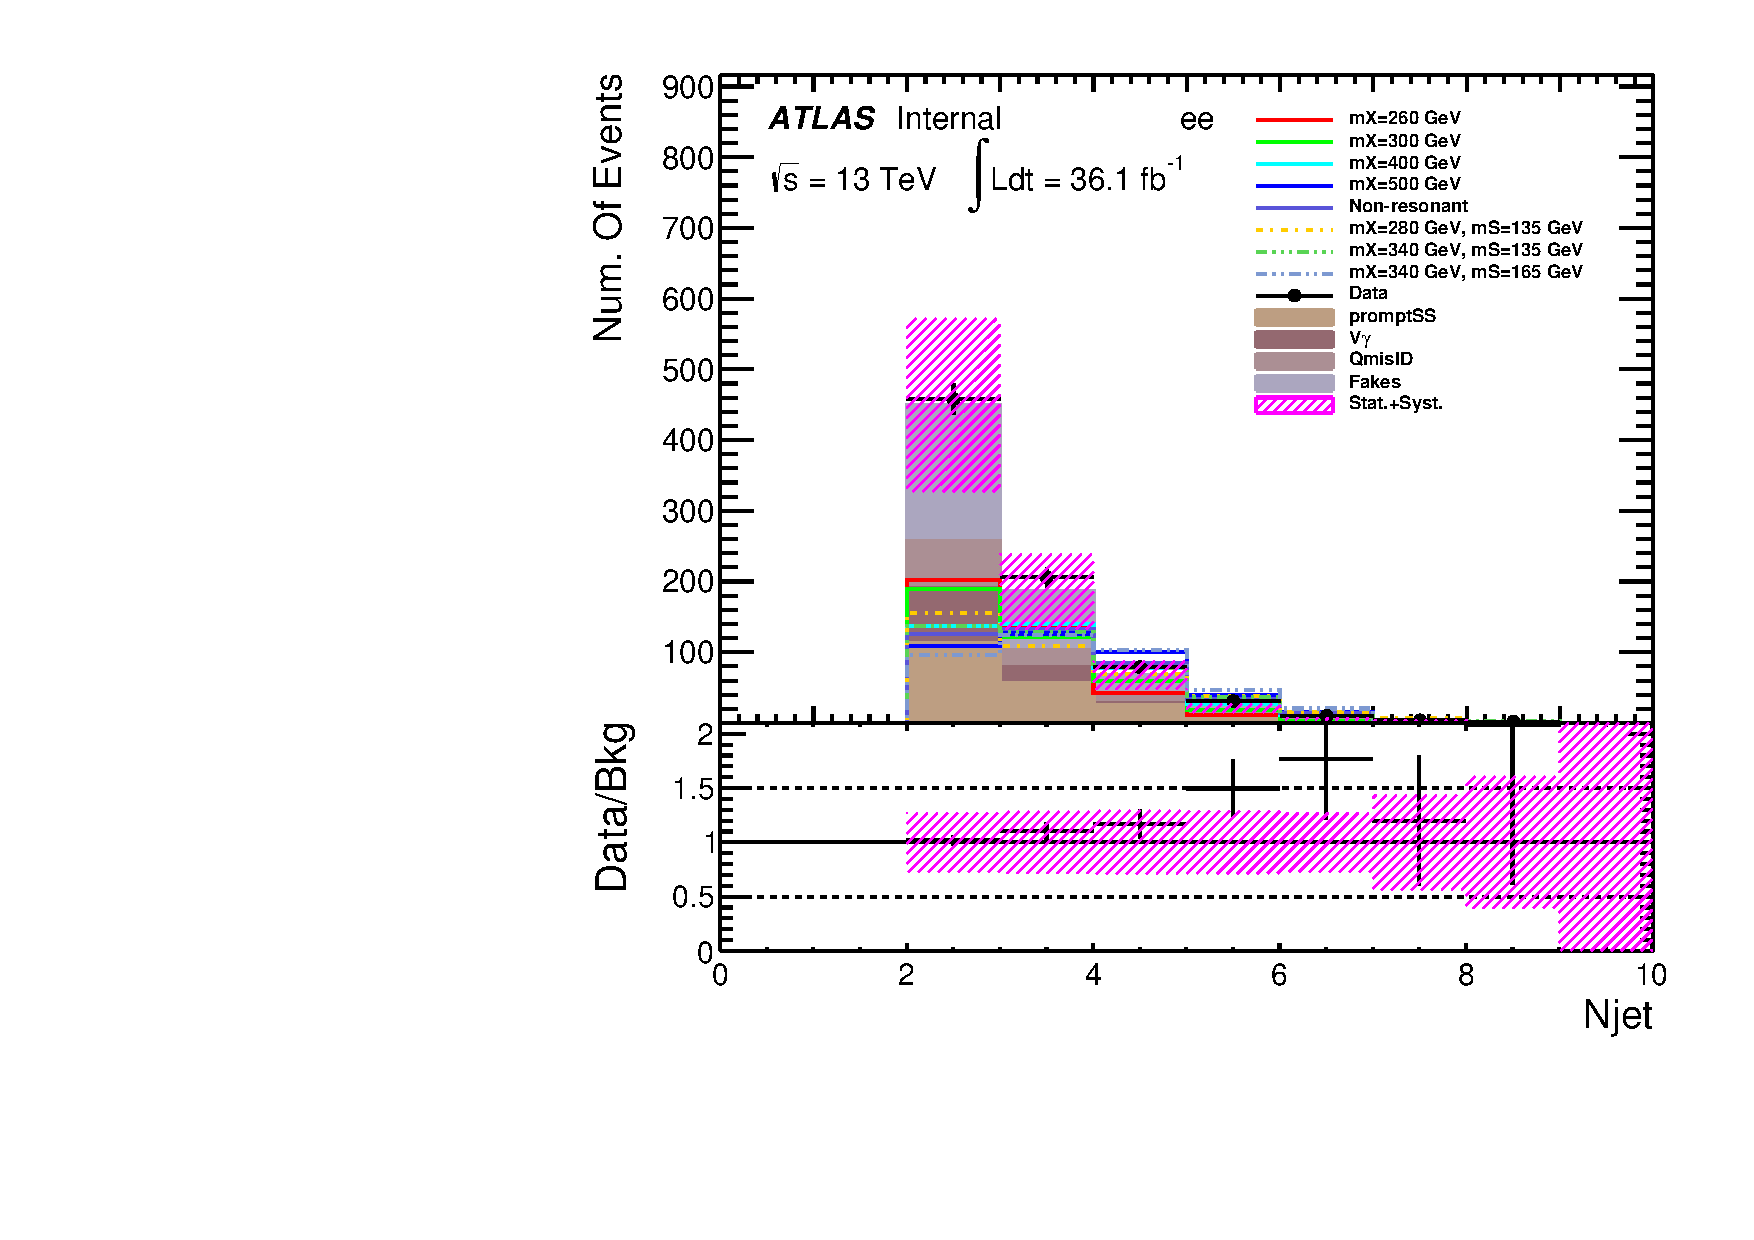
\includegraphics[width=1.0\textwidth,angle=-90]{fig/dataMC_low_Njet_CR/numOfjet_ee.pdf}
\end{minipage}
\begin{minipage}[t]{0.33\linewidth}
\centering
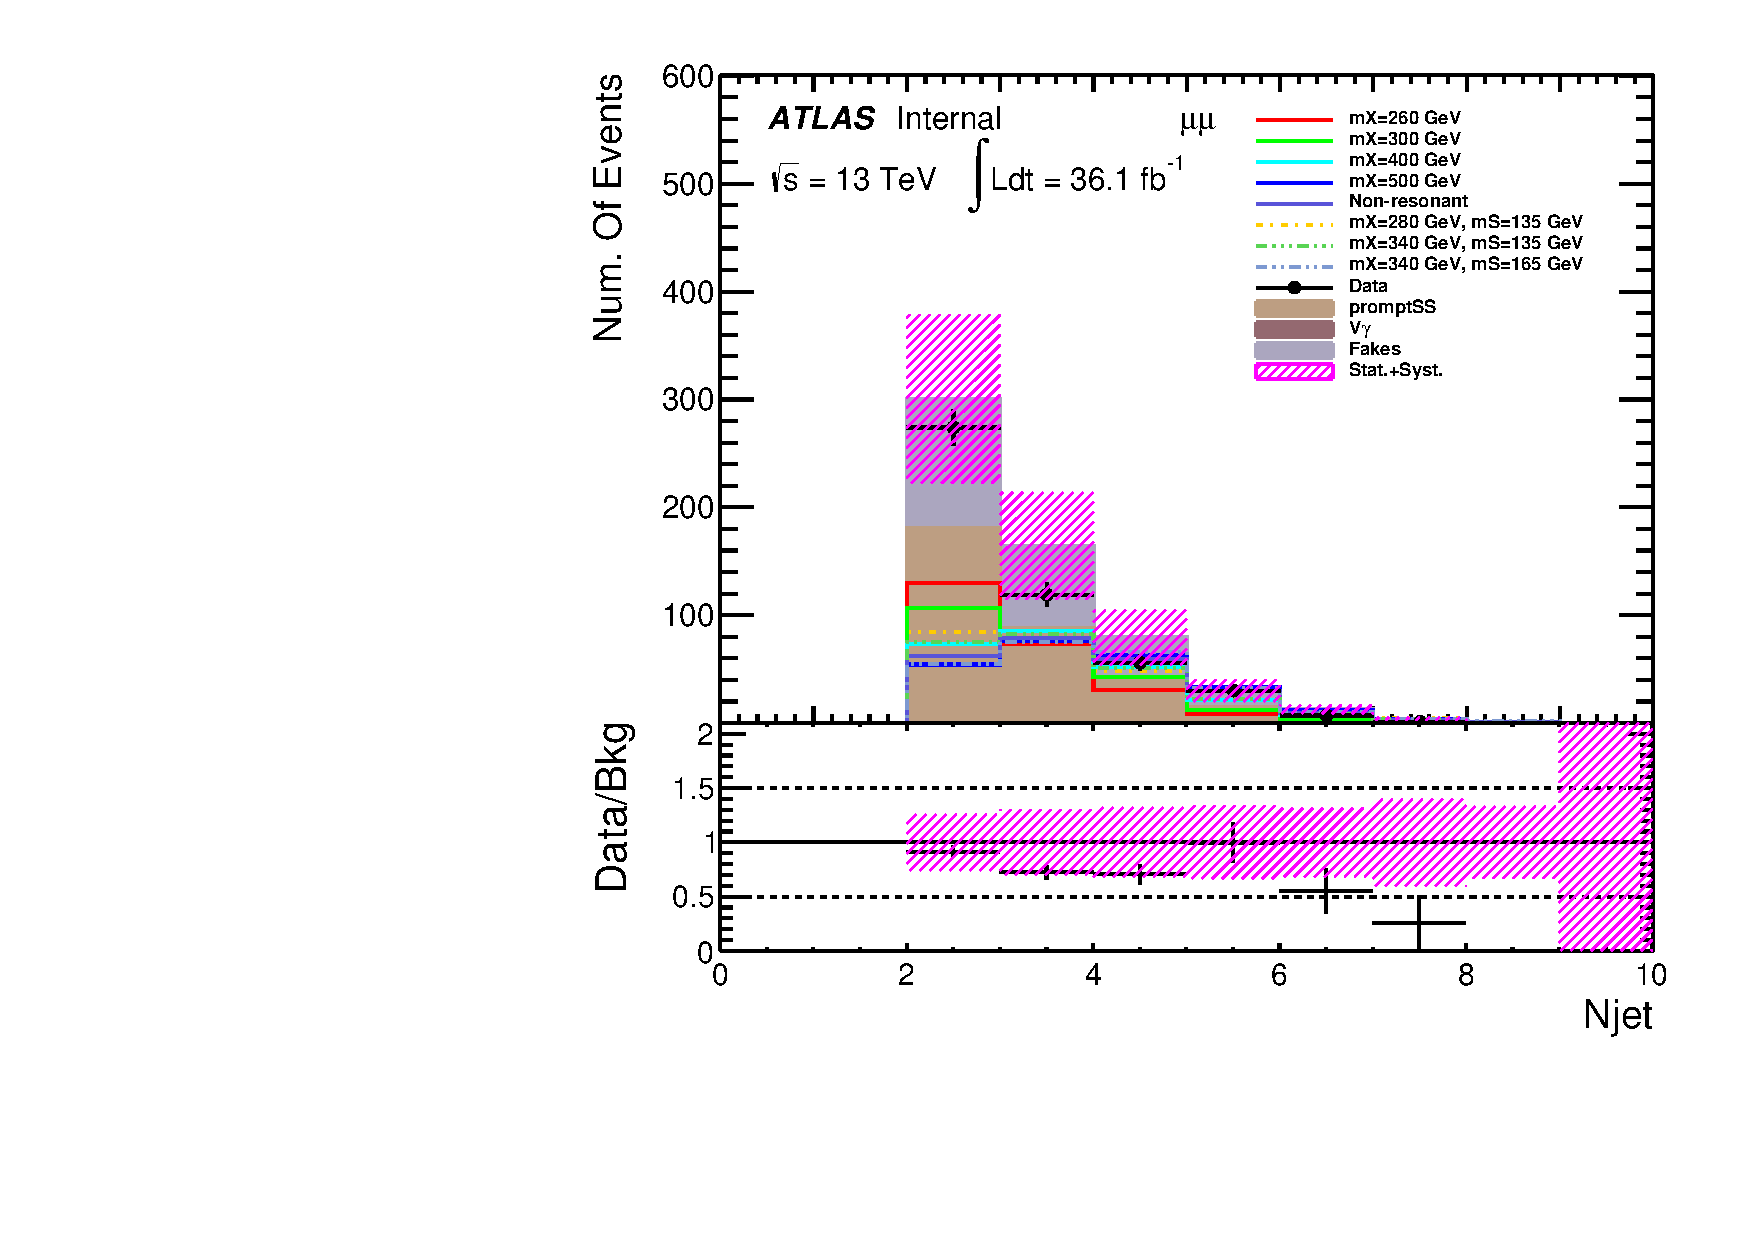
\includegraphics[width=1.0\textwidth,angle=-90]{fig/dataMC_low_Njet_CR/numOfjet_mumu.pdf}
\end{minipage}
\begin{minipage}[t]{0.33\linewidth}
\centering
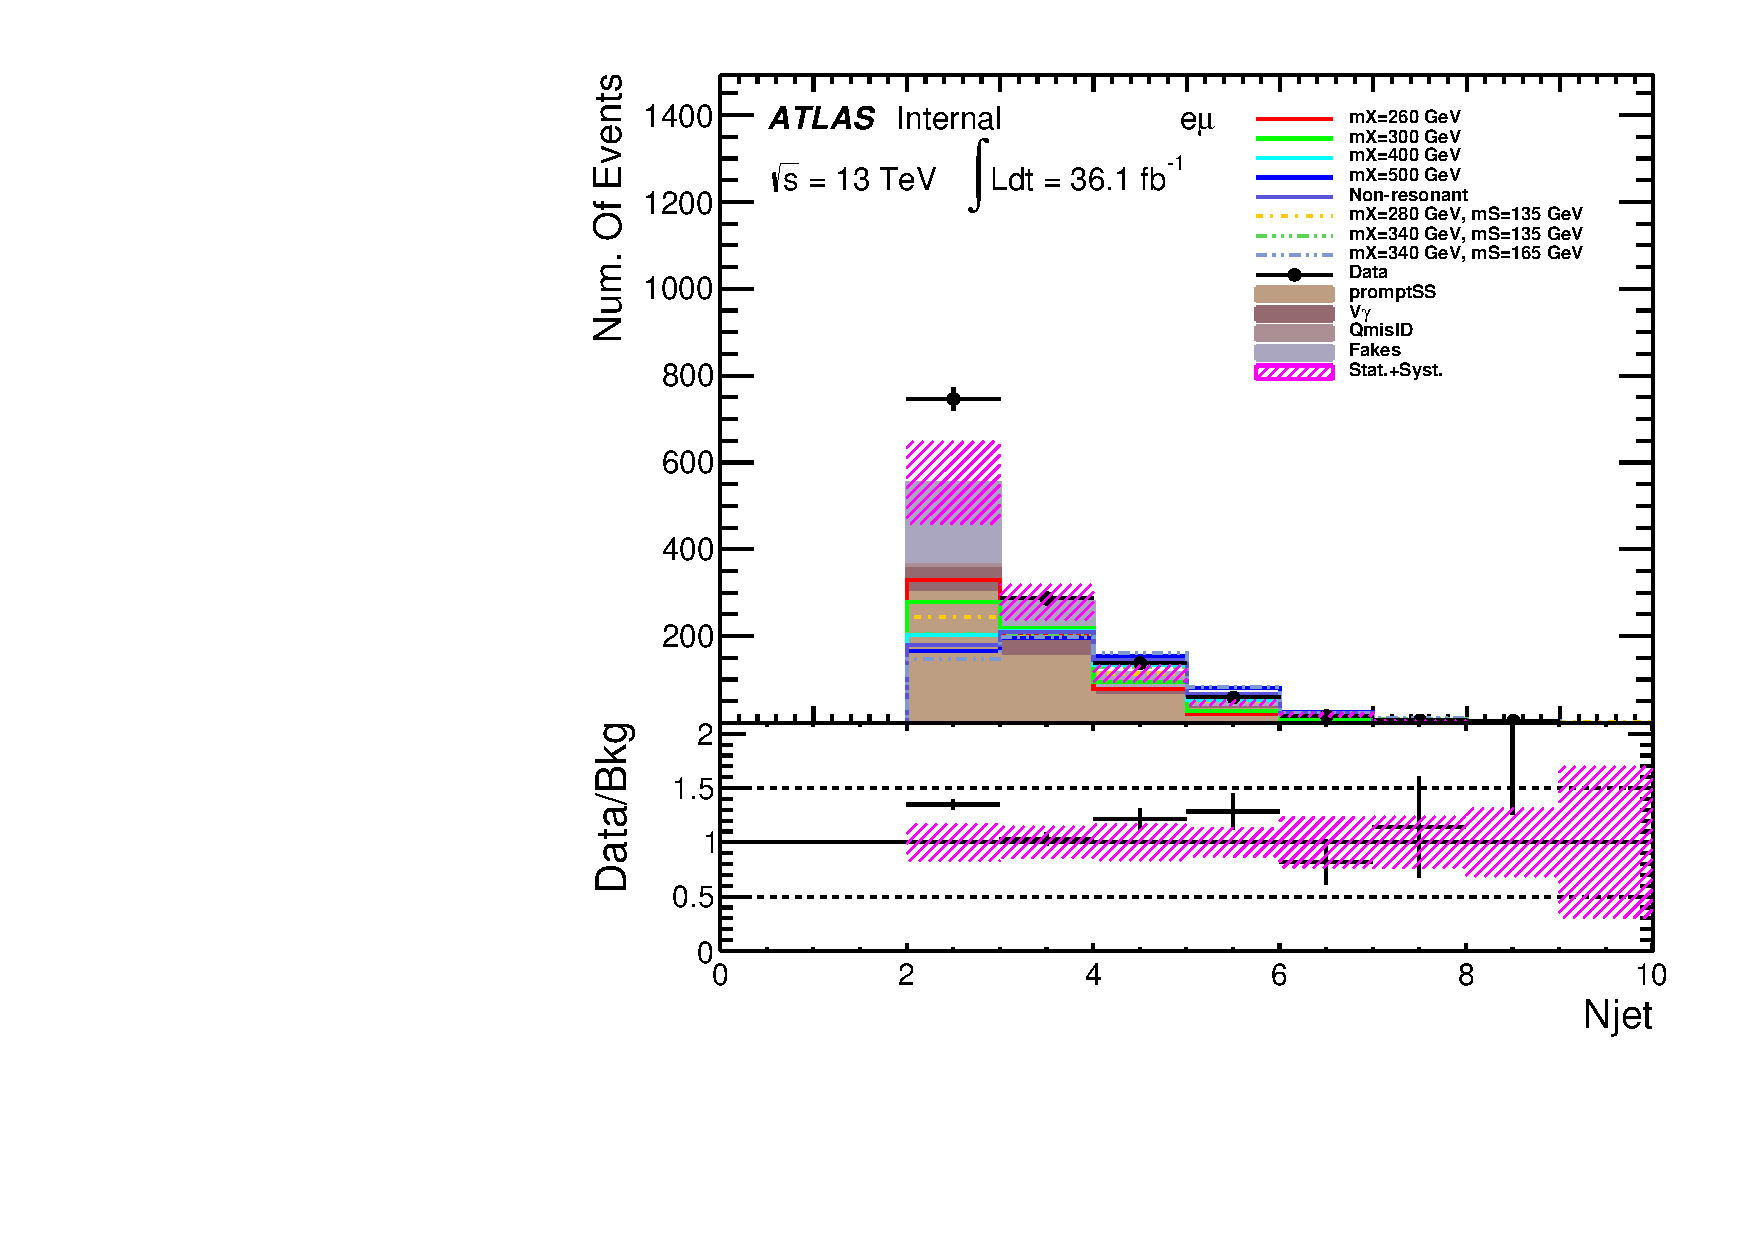
\includegraphics[width=1.0\textwidth,angle=-90]{fig/dataMC_low_Njet_CR/numOfjet_emu.pdf}
\end{minipage}
 \caption{The comparisons between data and backgrounds at pre-selection level, corresponding to $N_{\text{jet}}\geq2$. Left: $ee$, middle: $\mu\mu$, right: $e\mu$. The uncertainties, represented by slashed bands, include all systematics on fakes and statistical uncertainties on the other background components. PromptSS and $V+\gamma$ are normalized to the luminosity of 36.1 fb$^{-1}$.}
\label{fig:dataMC_low_Njet_CR:numOfjet}
\end{figure}

\begin{figure}[h]
\begin{minipage}[t]{0.33\linewidth}
\centering
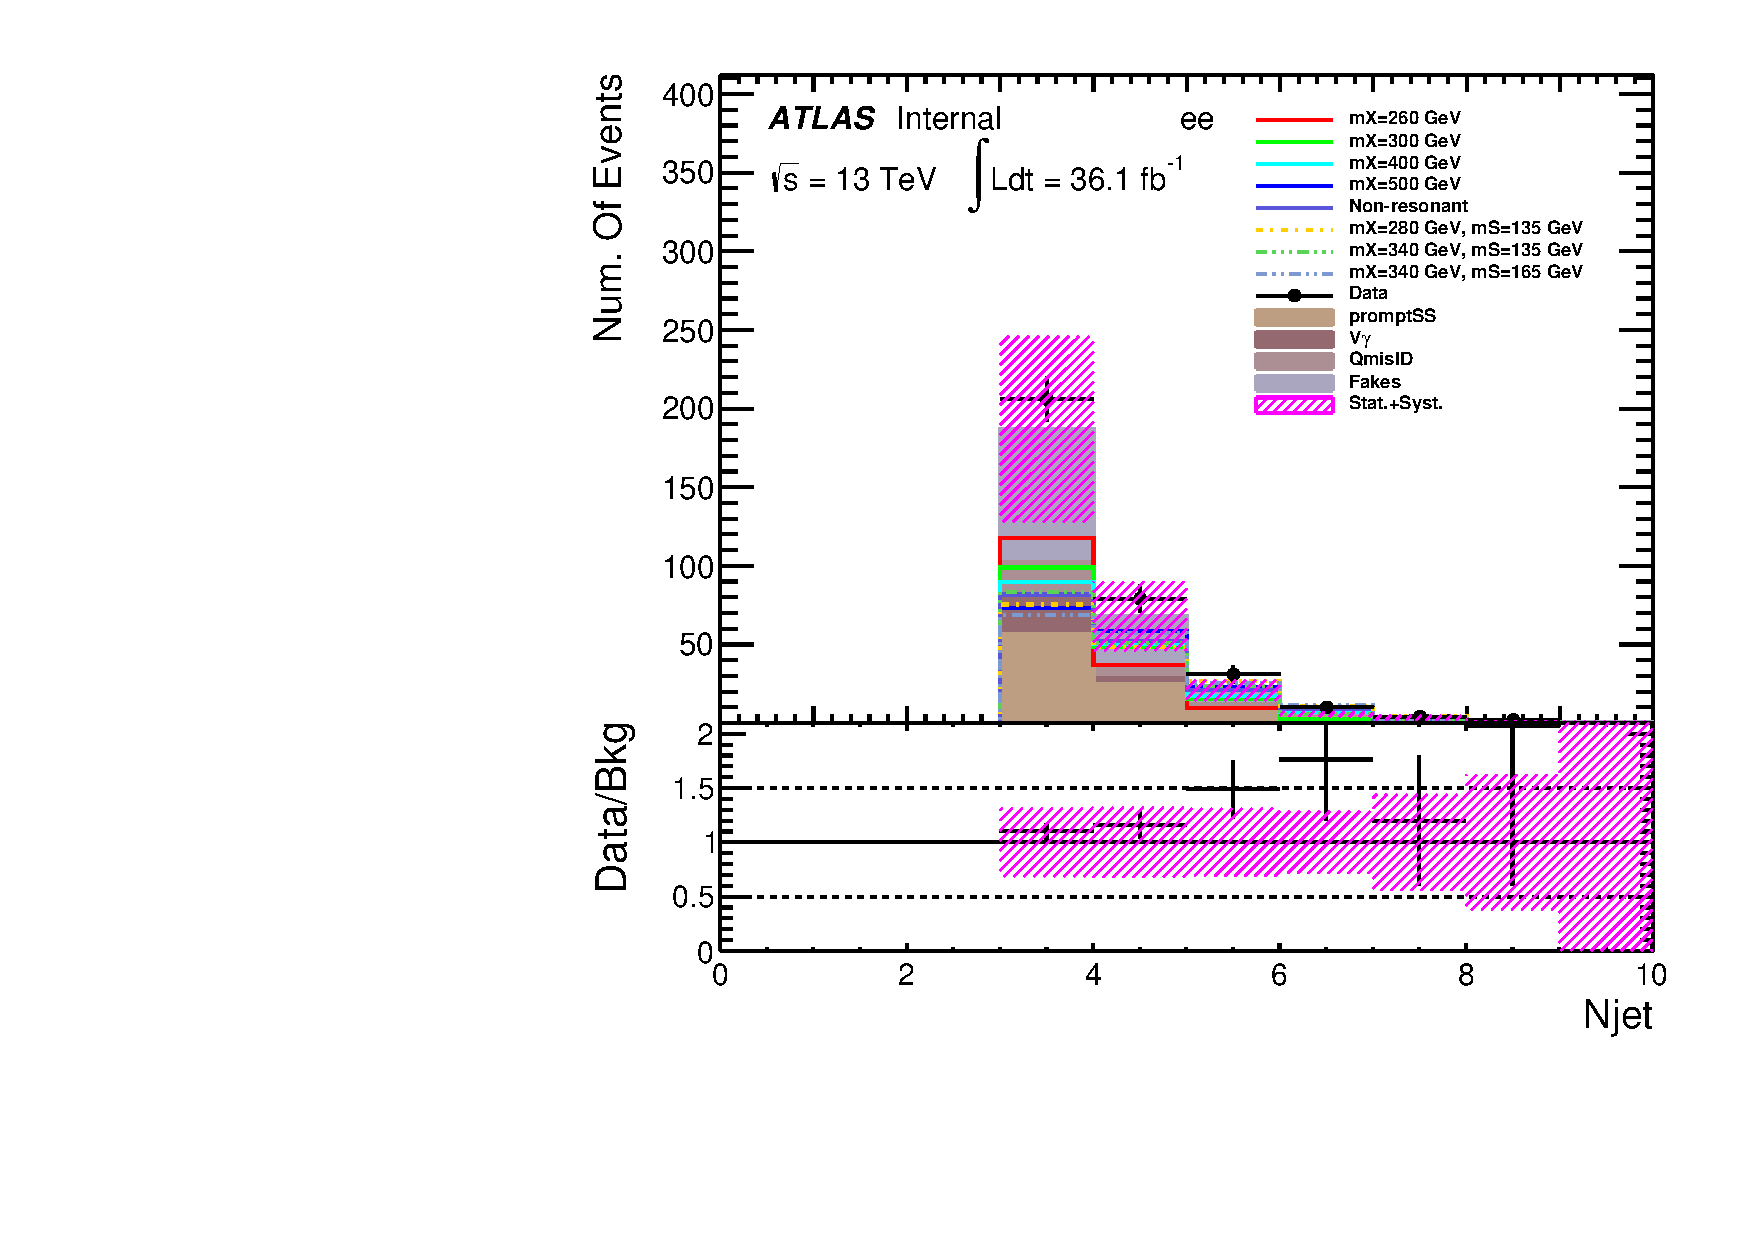
\includegraphics[width=1.0\textwidth,angle=-90]{fig/dataMC_high_Njet_CR/numOfjet_ee.pdf}
\end{minipage}
\begin{minipage}[t]{0.33\linewidth}
\centering
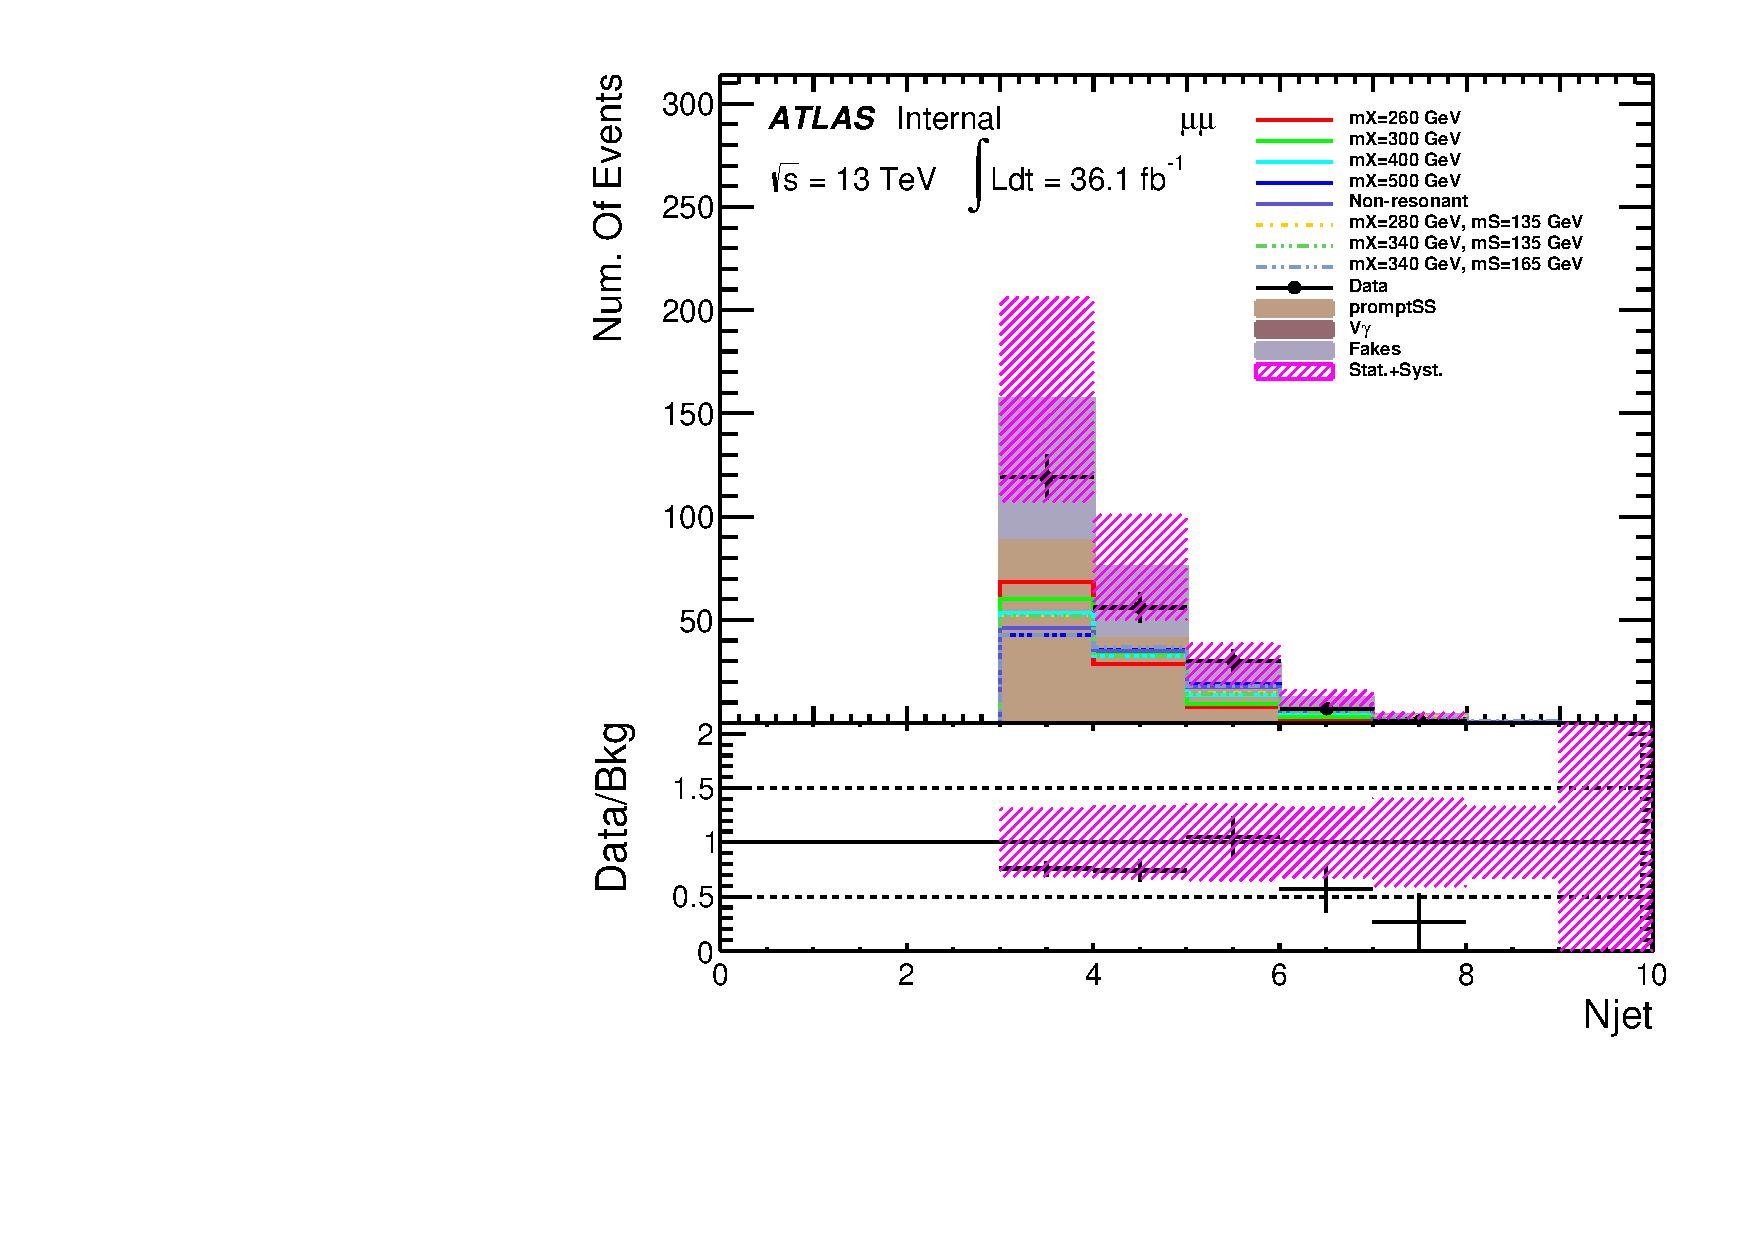
\includegraphics[width=1.0\textwidth,angle=-90]{fig/dataMC_high_Njet_CR/numOfjet_mumu.pdf}
\end{minipage}
\begin{minipage}[t]{0.33\linewidth}
\centering
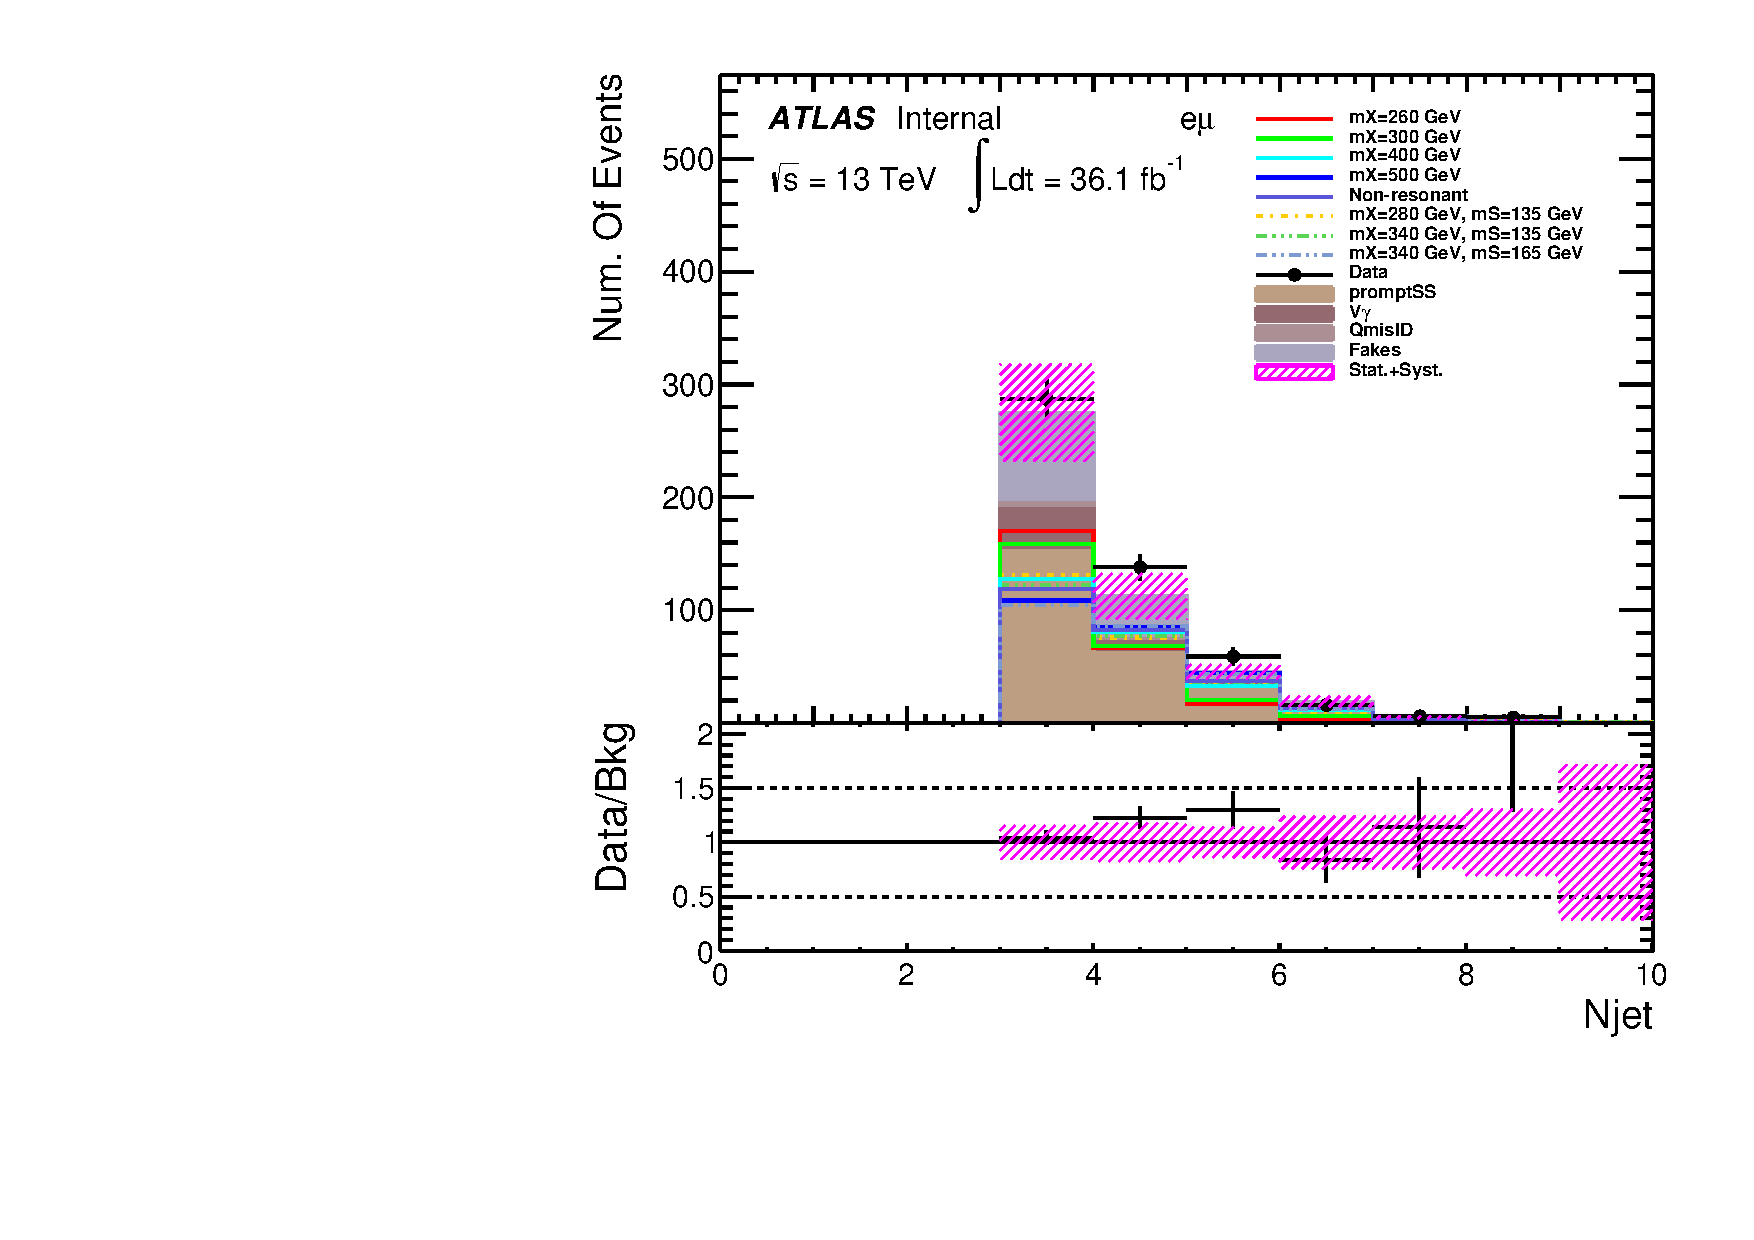
\includegraphics[width=1.0\textwidth,angle=-90]{fig/dataMC_high_Njet_CR/numOfjet_emu.pdf}
\end{minipage} \caption{The comparisons between data and backgrounds at pre-selection level, corresponding to $N_{\text{jet}}\geq3$. Left: $ee$, middle: $\mu\mu$, right: $e\mu$. The uncertainties, represented by slashed bands, include all systematics on fakes and statistical uncertainties on the other background components. PromptSS and $V+\gamma$ are normalized to the luminosity of 36.1 fb$^{-1}$.}
\label{fig:dataMC_high_Njet_CR:numOfjet}
\end{figure}
